\chapter{The Resonance Search on the Dimuon Signature}
\label{chapter:dimuon}

\section{Introduction}

    % Why this is interesting  
    Owing to its unprecedented high energy, the run I and early run II of ATLAS has long focused on the high mass resonances searches. This has left some gaps in the low mass region that are unexplored. In the two lepton final state, there has been an analysis after the Z boson peak since the beginning of Run 1, however the mass region below the Z mass peak has left a region totally uncovered on ATLAS.

\begin{figure}[!htb]
    \begin{center}
        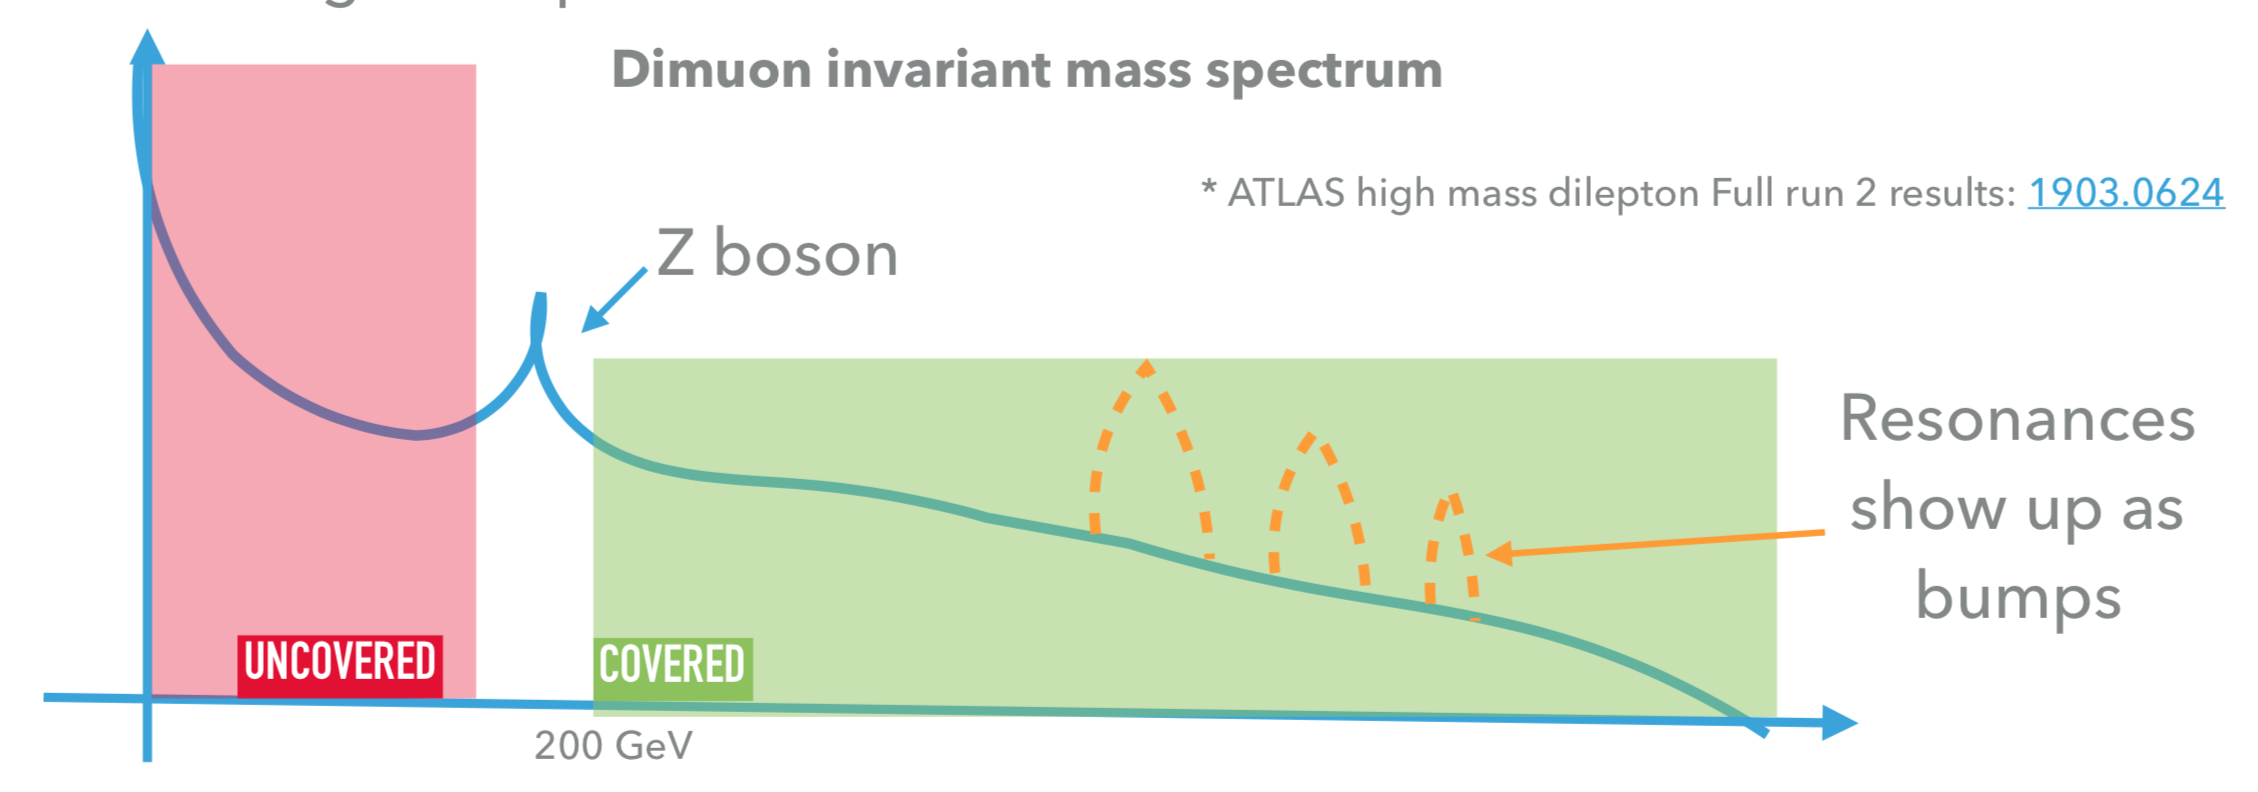
\includegraphics[width=0.75\textwidth]{figures/chapter_dimuon/dimuonStudies}        
        \caption{
        This cartoon illstrate the target signal region of the analysis and how it has not been covered by the previous high-mass dilepton analysis. }
            \label{fig:dimuonstudies}
    \end{center}
\end{figure}
   
    Since ATLAS collide partons, there are fewer background on leptons than jet processes, this allows lower transverse momentum lepton events to be saved. Using two muons as the resonance final state items, lower mass resonances can be searched for, going below the limits of the dijet resonances. The signal significance would be higher compared to jet. 

    This search results is interesting to the theoretical community for the dark matter benchmark interpretation possible.

%\section{Historical searches}    
%    Previous searches has been done directly in Tevatron experiment. Indirect constraints has been made in LEP as well. 
%
%    CMS results and tevatron results: 
%    
%    This study will be an independent finding from ATLAS and the first search done in this region.  


\section{The Search Channels}
Since there is a trigger turn-on feature near 45 GeV in the distribution due to the cut in muon transverse momentum in trigger, 
This analysis is based on a pheno-study first done here\cite{2014}.

There are two search channels in the analysis, each covering a different mass region, namely the boosted and the 

\begin{figure}[!htb]
    \begin{center}
        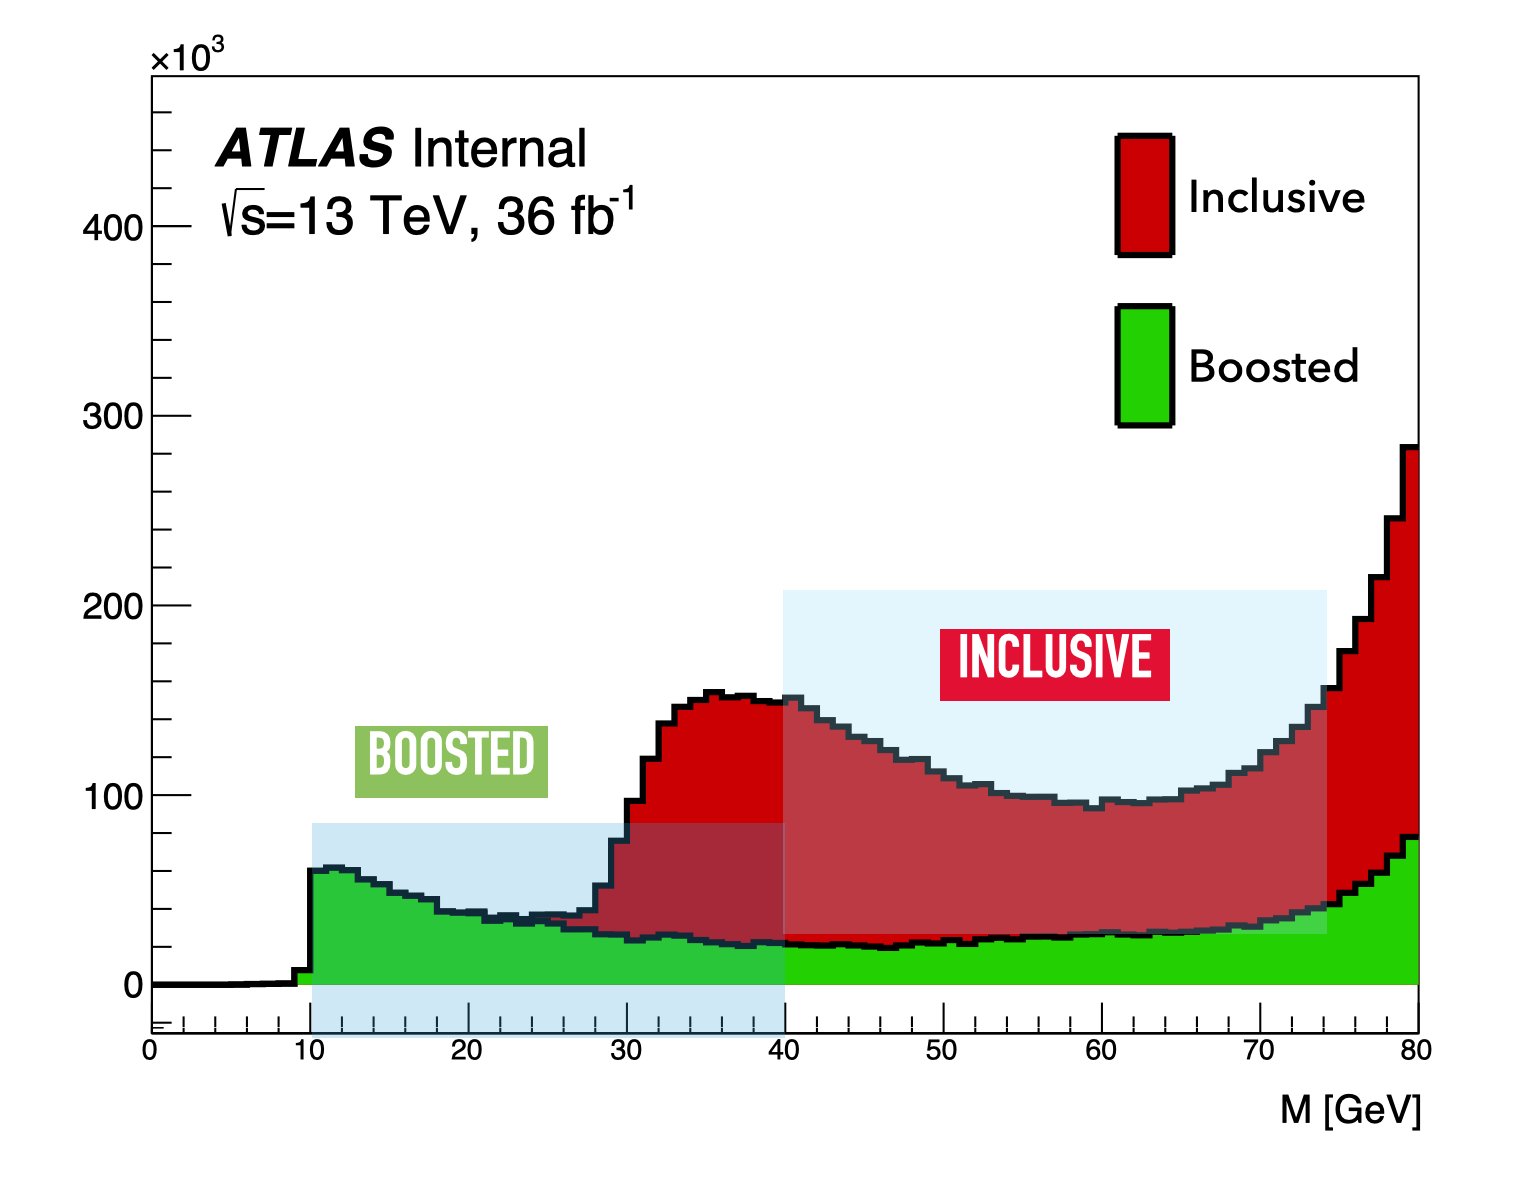
\includegraphics[width=0.75\textwidth]{figures/chapter_dimuon/turnon}
        \caption{
        this figure shows the trigger turn on curve in the inclusive dimuon channel, and how utilizing the boosted channel a smooth background is possible in the lower mass region from 10-45 gev. samples used here are from the monte carlo sample in section~\ref{}, a minimal cut of muon pt >14 gev are done on the two leading muons. }
            \label{fig:turnon}
    \end{center}
\end{figure}

\section{Signal Theoretical Model}

    The analysis uses the dark matter LHC benchmark model and dark photon model outlined in~\ref{sec:LHCDM}.
Other models that are of interest and can be searched for in this analysis includes the W', the quantum blackholes,and axion models. 
The following search focuses on the search on the vector dilepton signature from the dark photon model and the dark matter benchmark. But as Gaussian limits are also set, the results will be reinterpretable for many other models that predicts scalar or axion-vector resonances. 

\begin{figure}[!htb]
    \begin{center}
        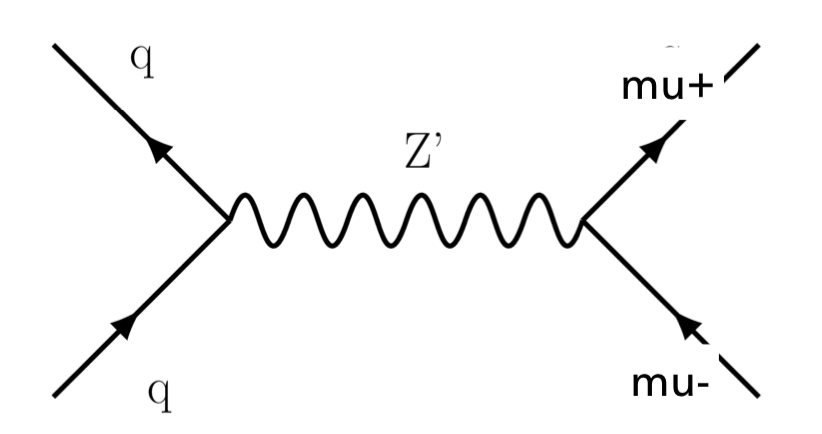
\includegraphics[width=0.75\textwidth]{figures/chapter_dimuon/dimuonFeynman}
        \caption{
            This figure shows the Feynmann diagram of the inclusive dimuon signal as the signal for the analysis. }
            \label{fig:dimuonFeynmann}
    \end{center}
\end{figure}


\begin{figure}[!htb]
    \begin{center}
        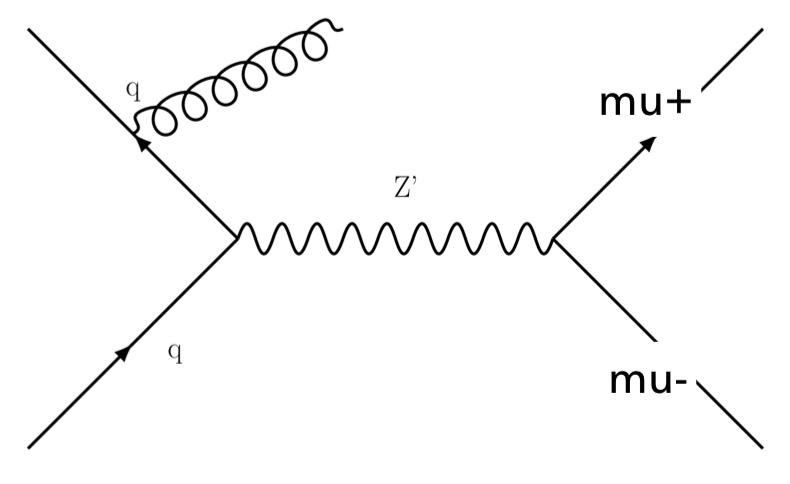
\includegraphics[width=0.75\textwidth]{figures/chapter_dimuon/dimuonISRFeynmann}
        \caption{
        This figure shows the Feynmann diagram of the boosted dimuon ISR signa used as the signal for the analysis. }
            \label{fig:dimuonFeynmann}
    \end{center}
\end{figure}

    The different signal distributions across different kinematics are shown here. 

\begin{figure}[!htb]
    \begin{center}
        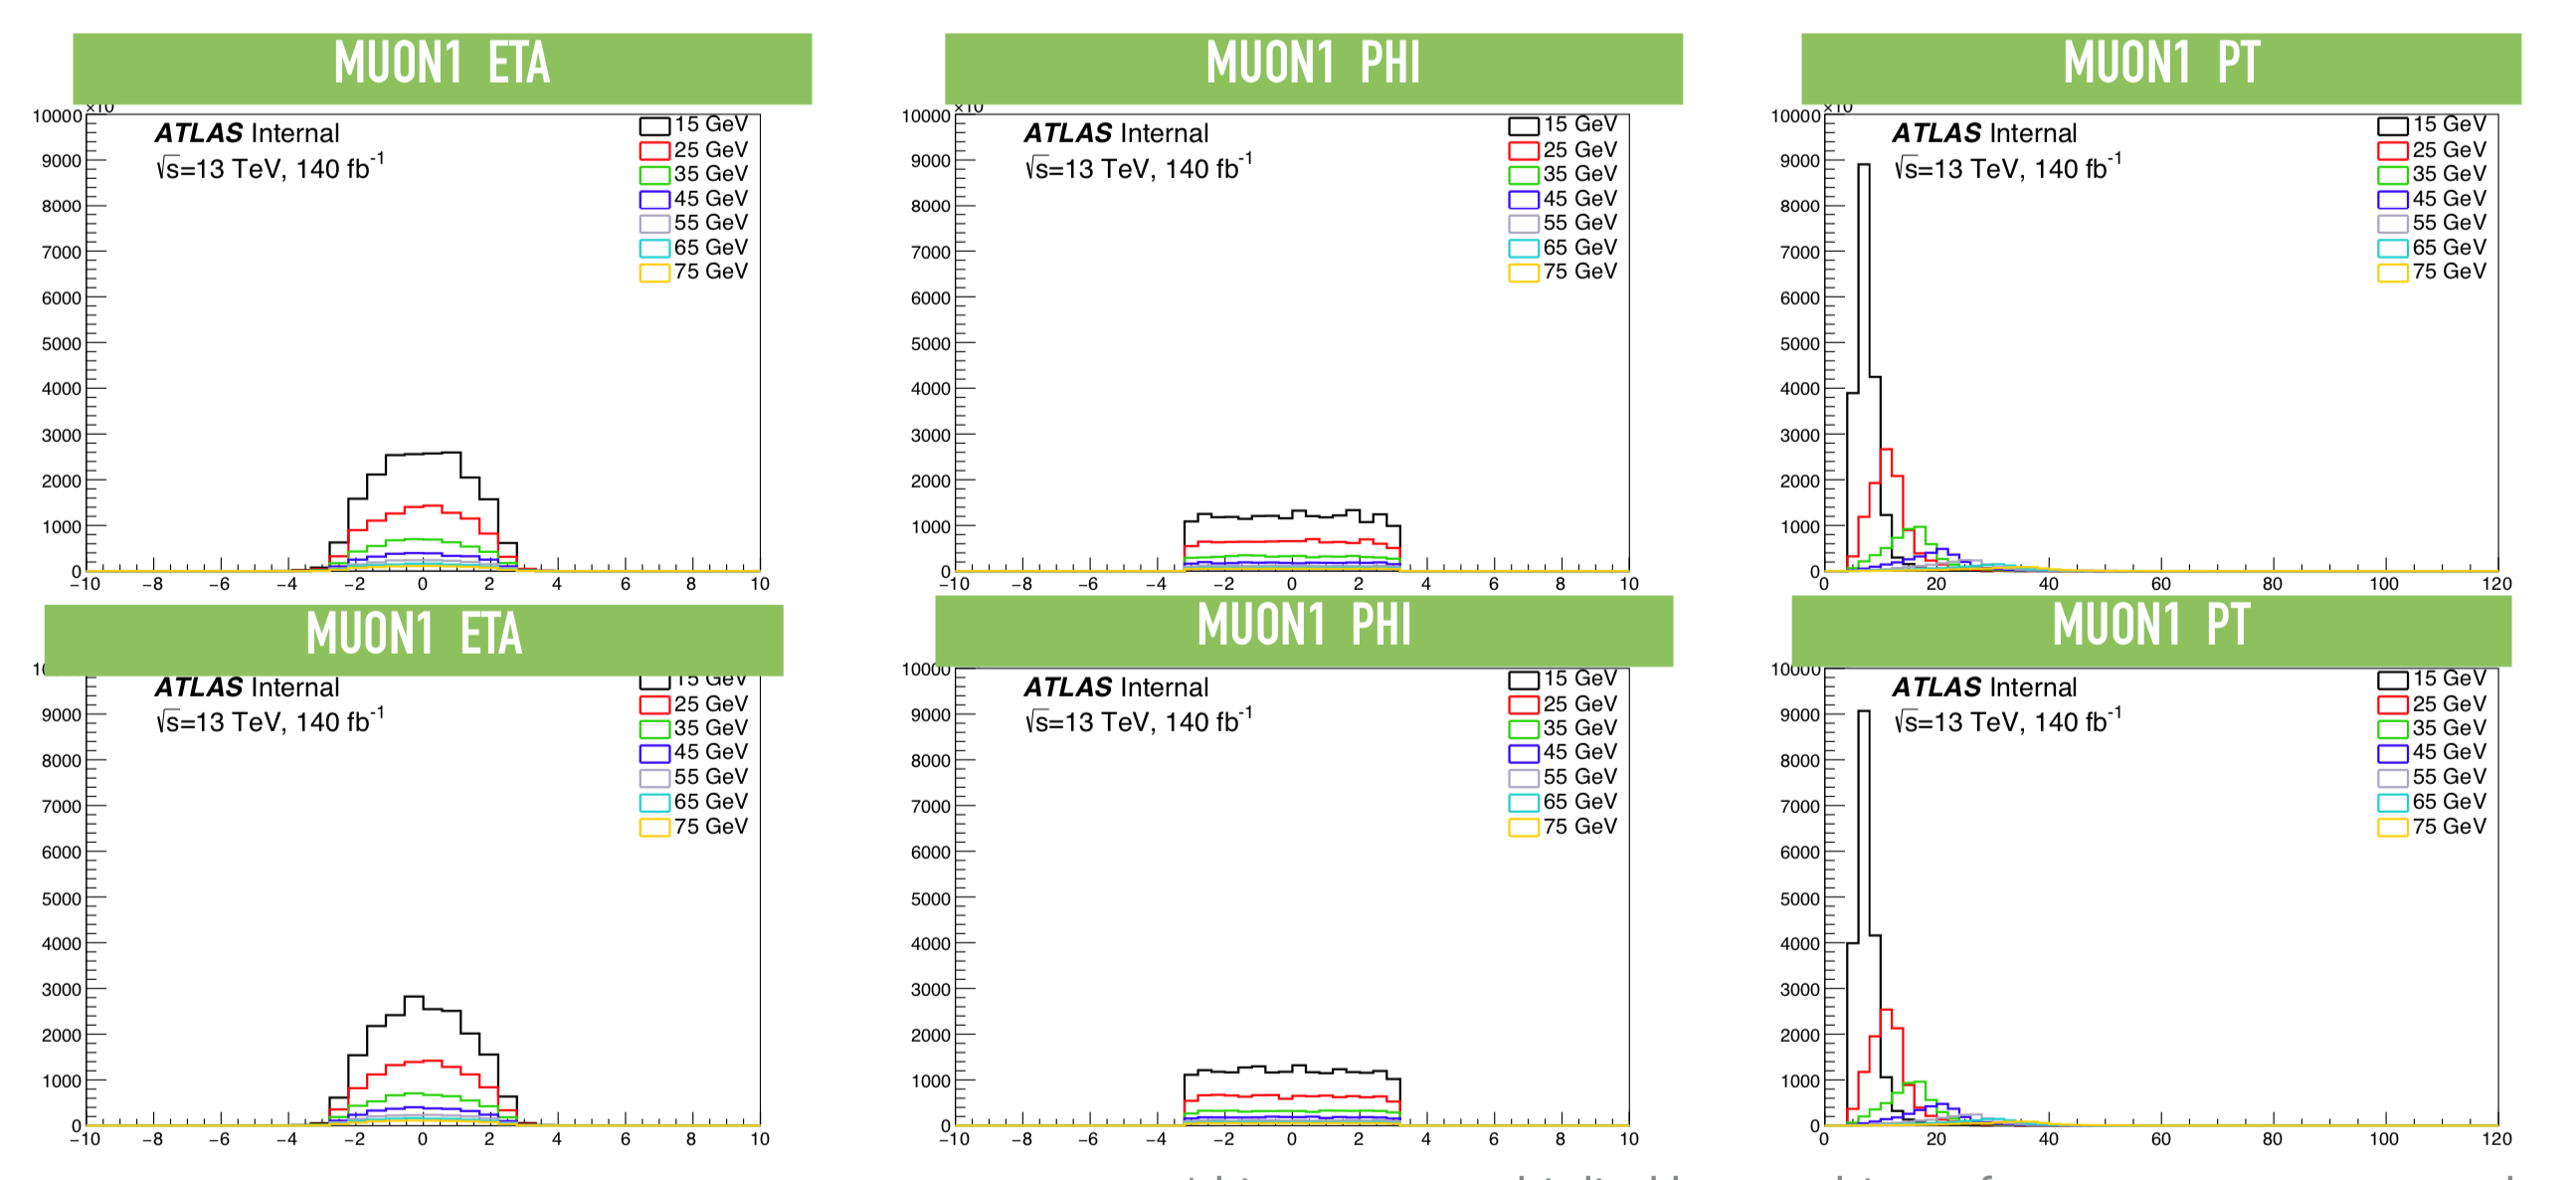
\includegraphics[width=0.75\textwidth]{figures/chapter_dimuon/dimuondist1}
        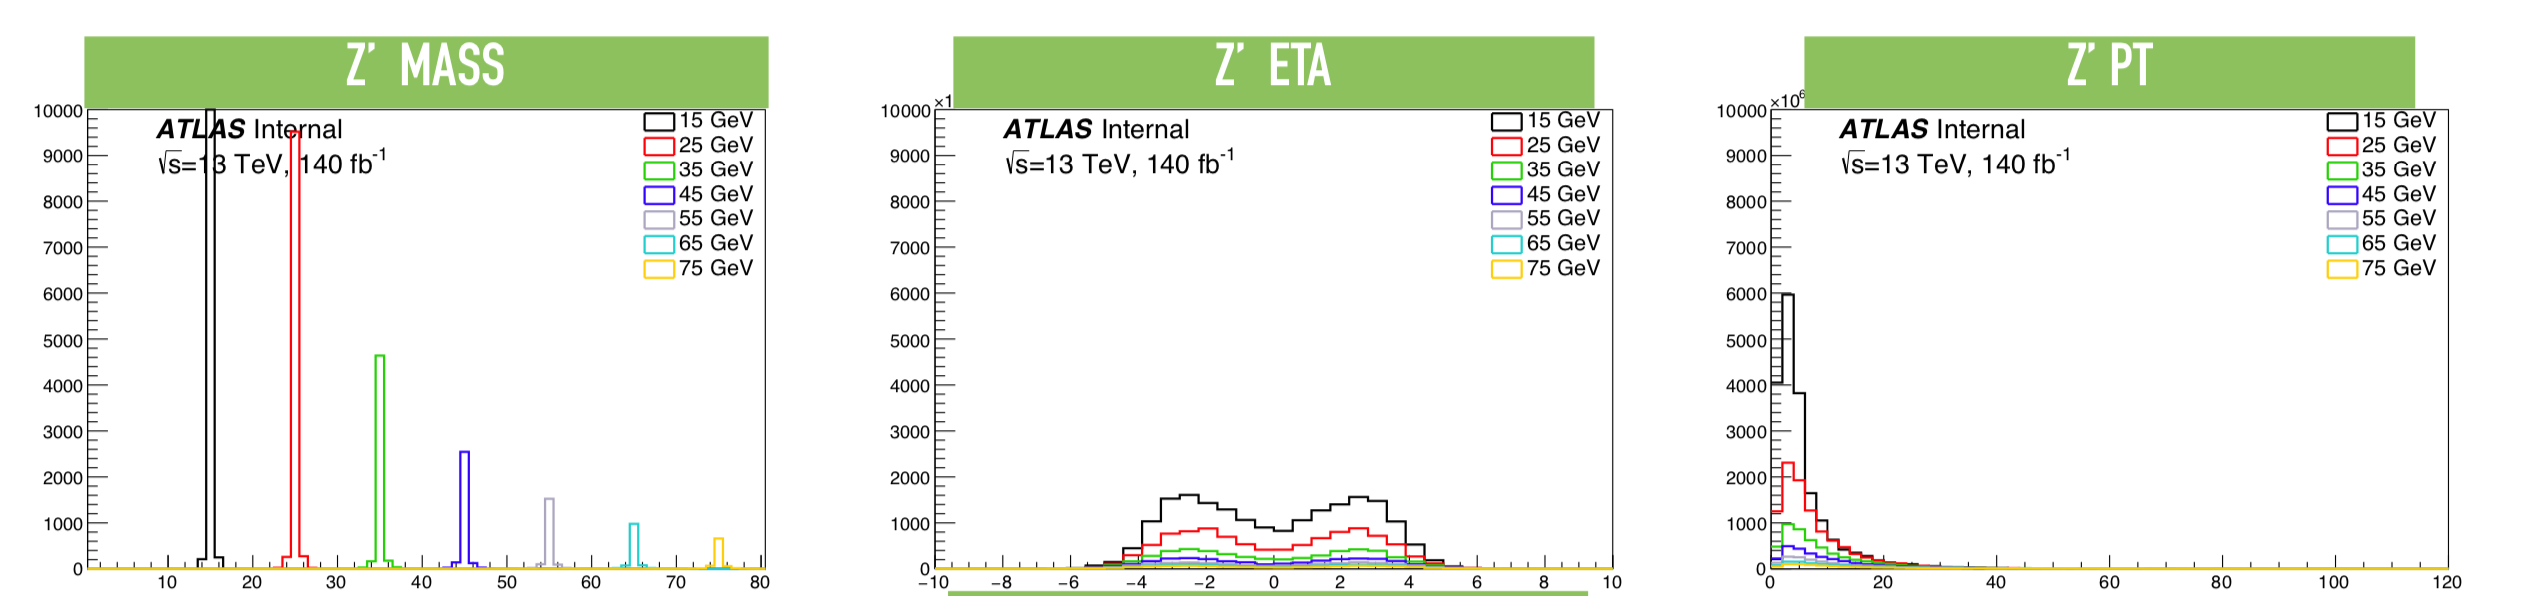
\includegraphics[width=0.75\textwidth]{figures/chapter_dimuon/dimuondist2}
        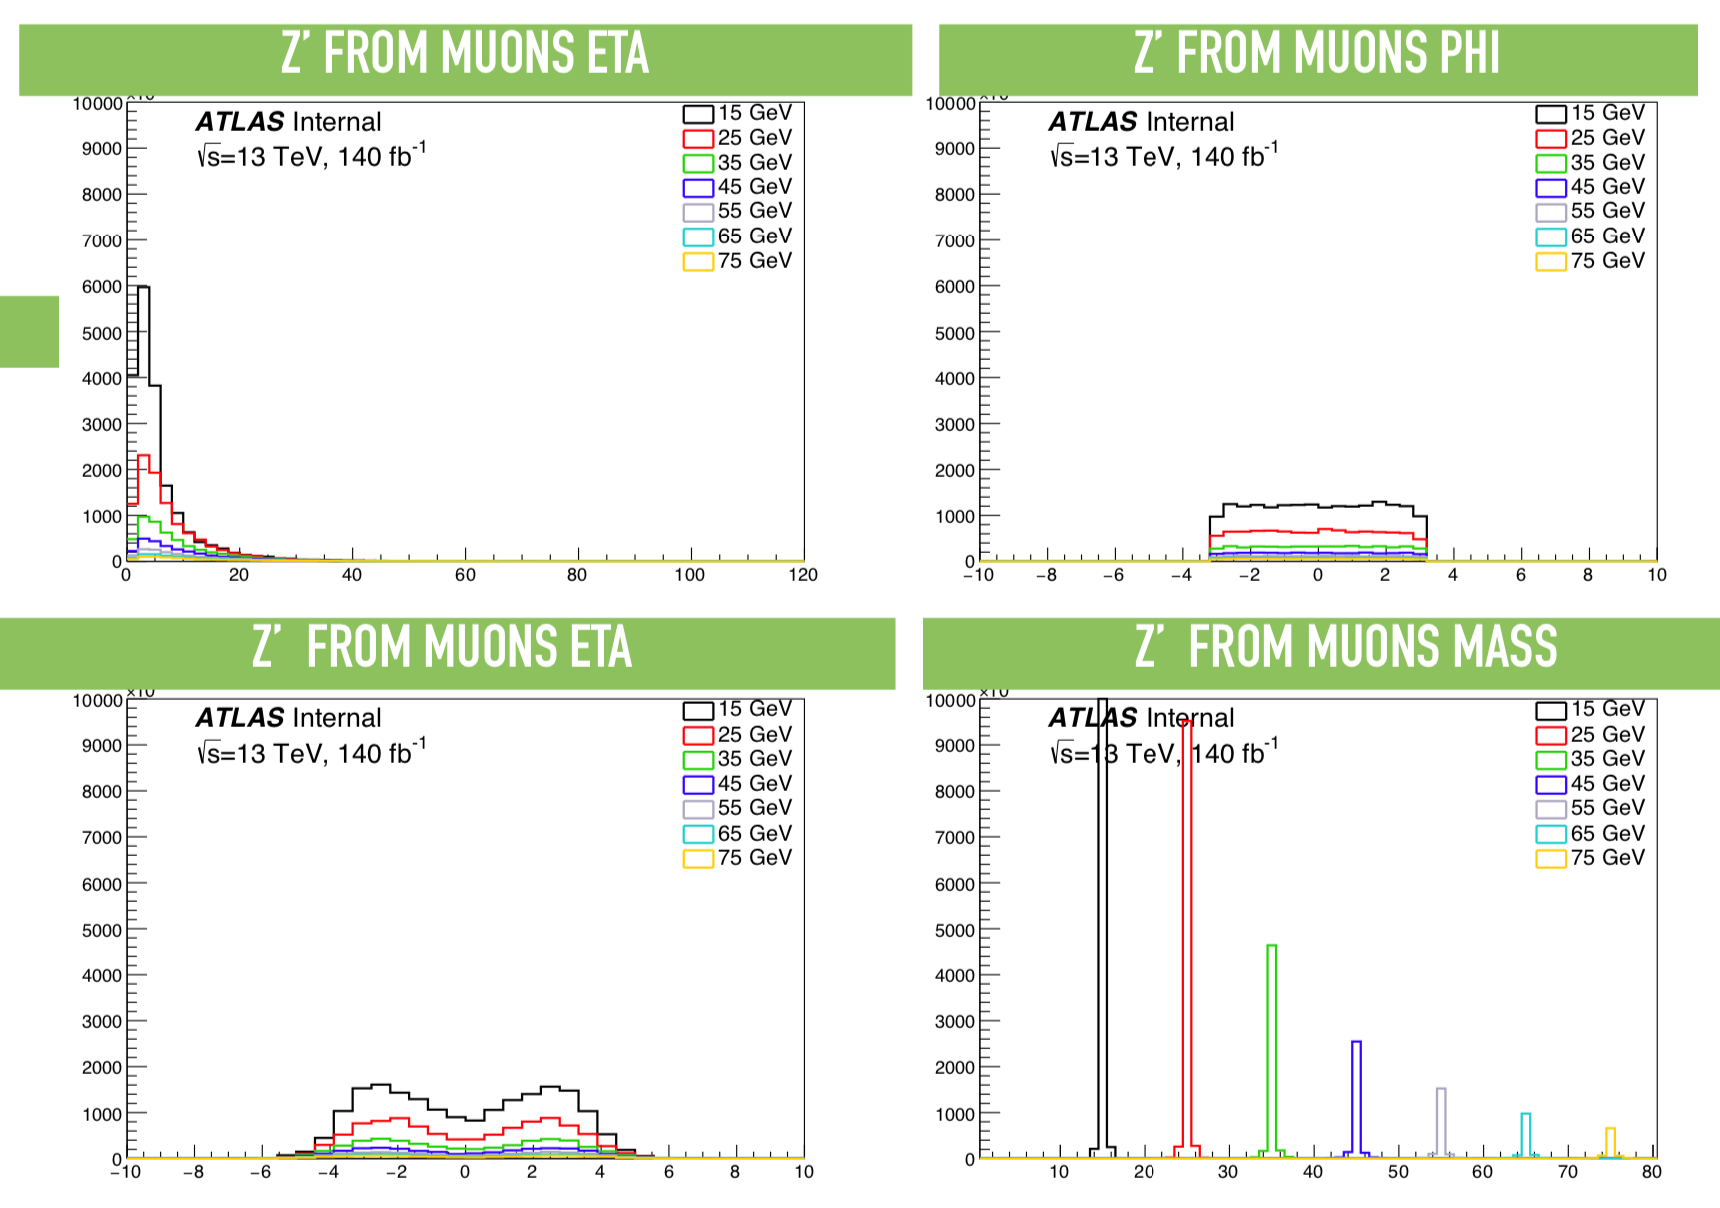
\includegraphics[width=0.5\textwidth]{figures/chapter_dimuon/dimuondist3}
        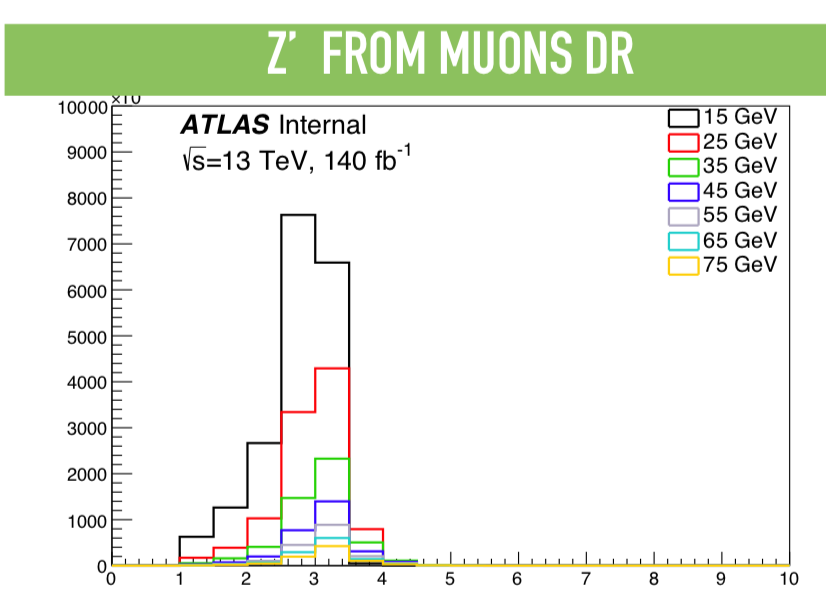
\includegraphics[width=0.2\textwidth]{figures/chapter_dimuon/dimuondist4}
        \caption{
        This figure shows the signal distribution of the inclusive dimuon samples generated. A minimal cut of muon pt >14 gev are done on the two leading muons. }
        \label{fig:dimuon}
    \end{center}
\end{figure}


\begin{figure}[!htb]
    \begin{center}
        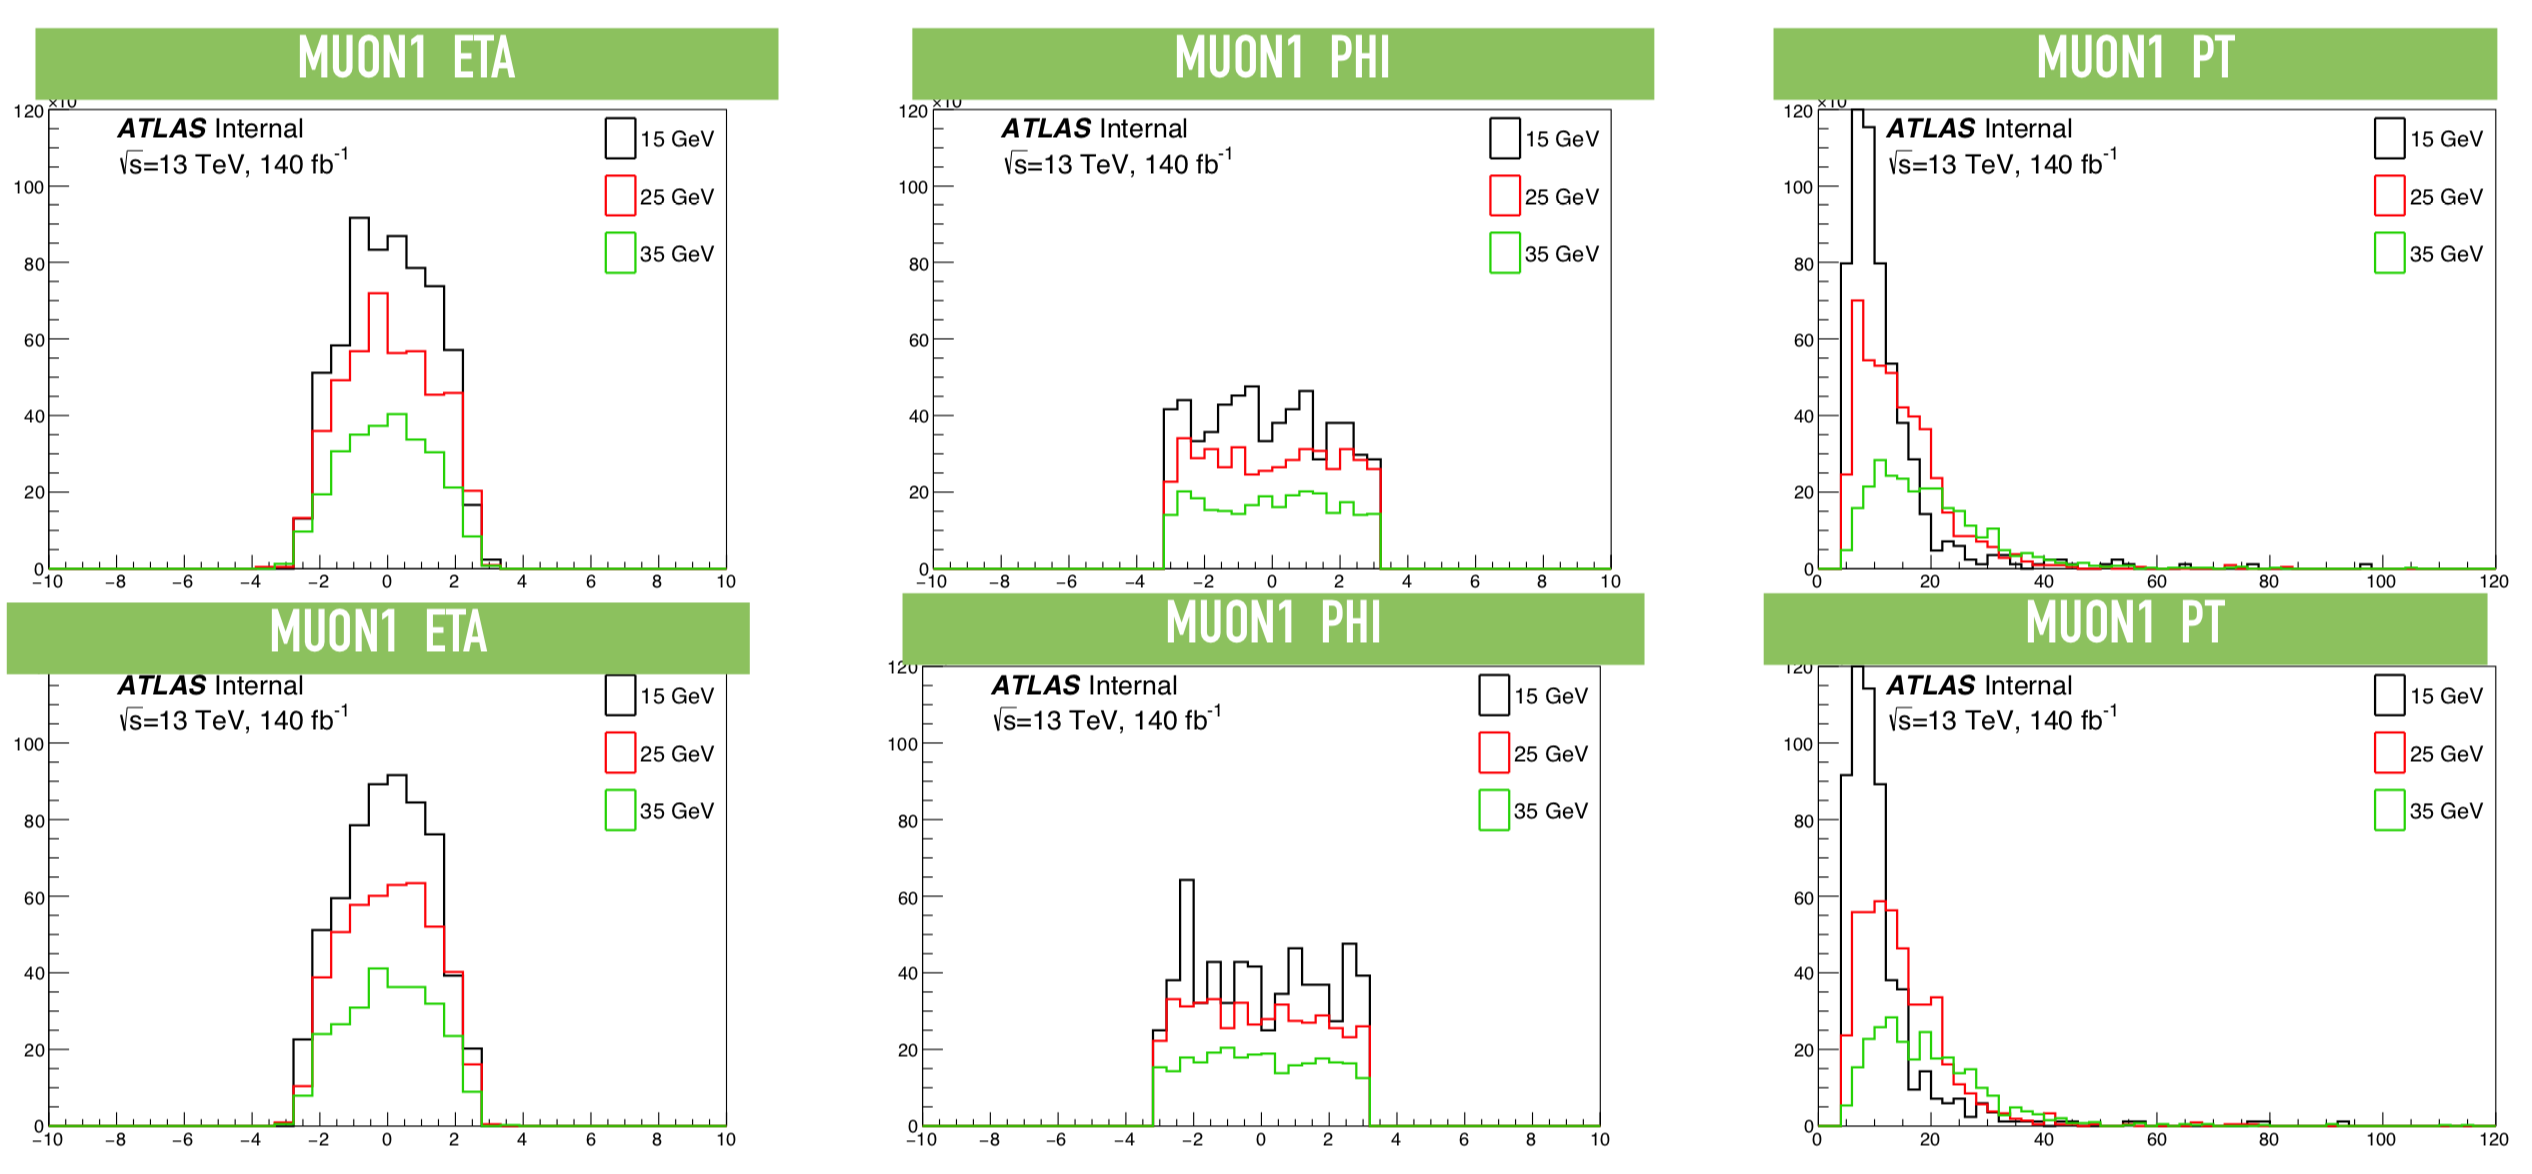
\includegraphics[width=0.75\textwidth]{figures/chapter_dimuon/dimuonISRdist1}
        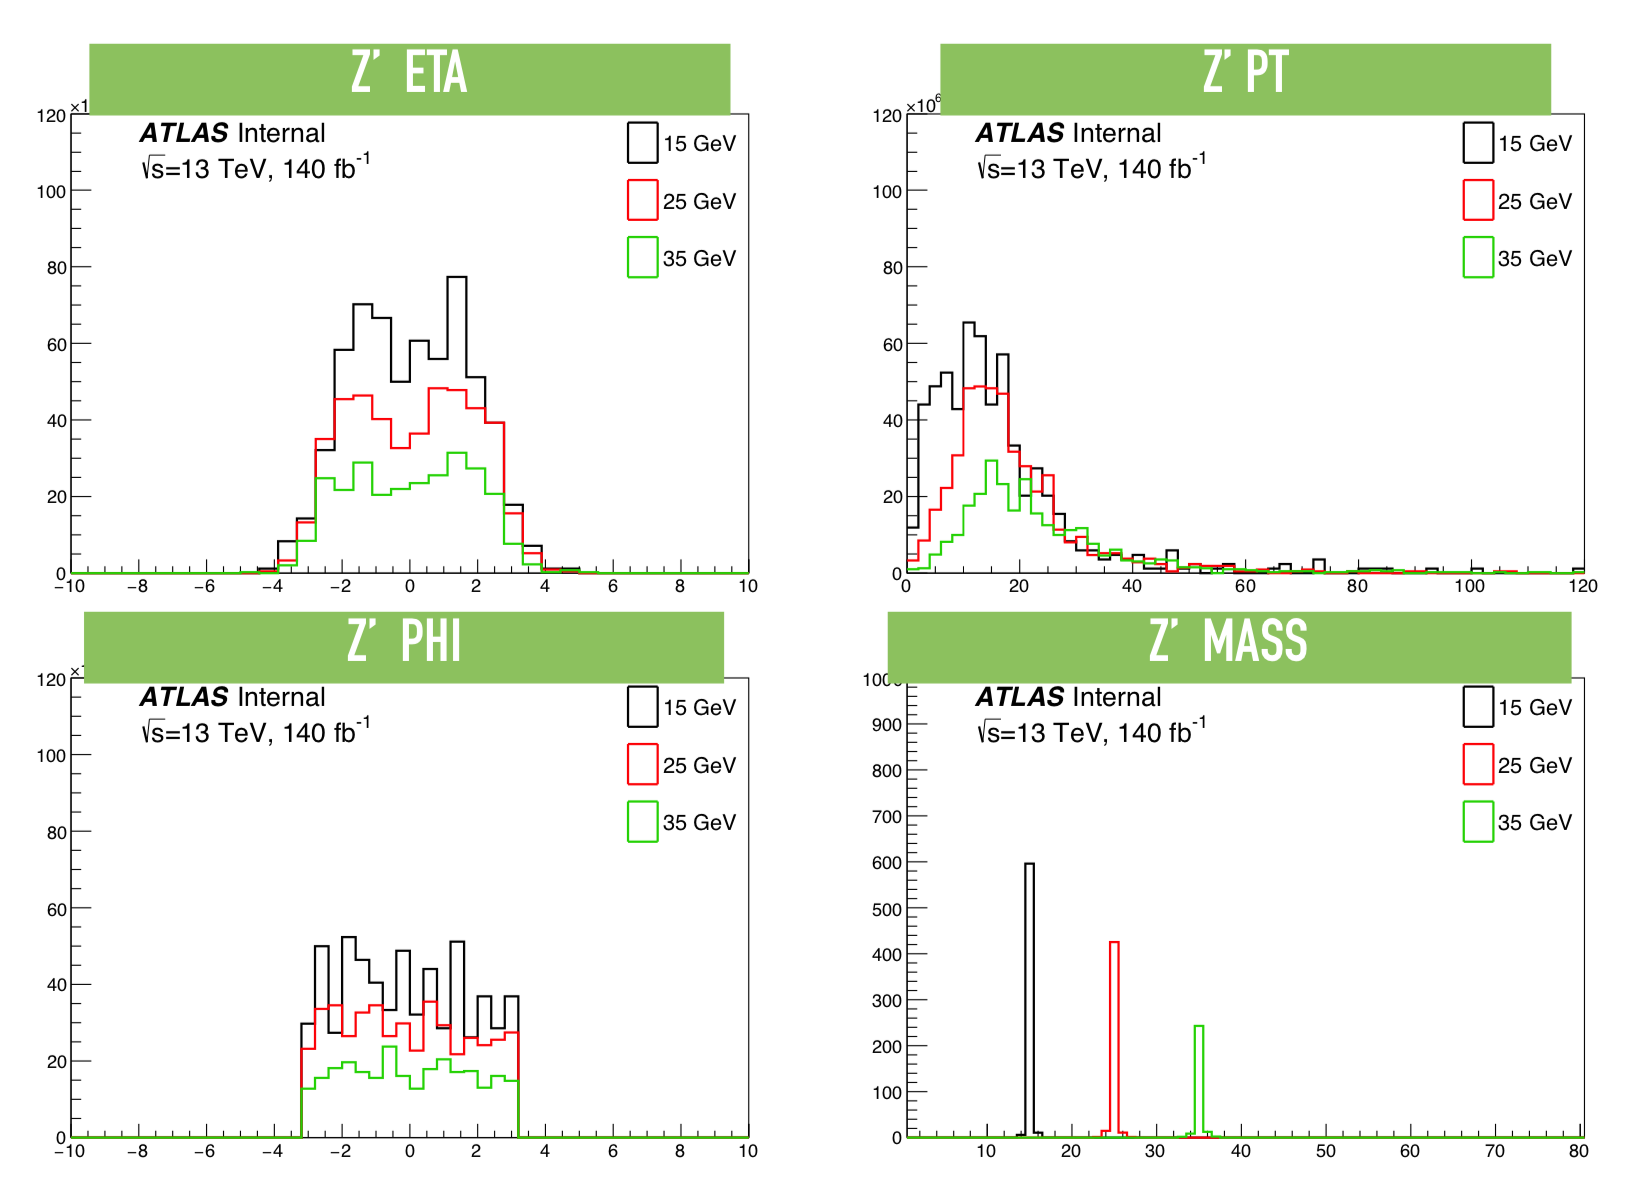
\includegraphics[width=0.5\textwidth]{figures/chapter_dimuon/dimuonISRdist2}
        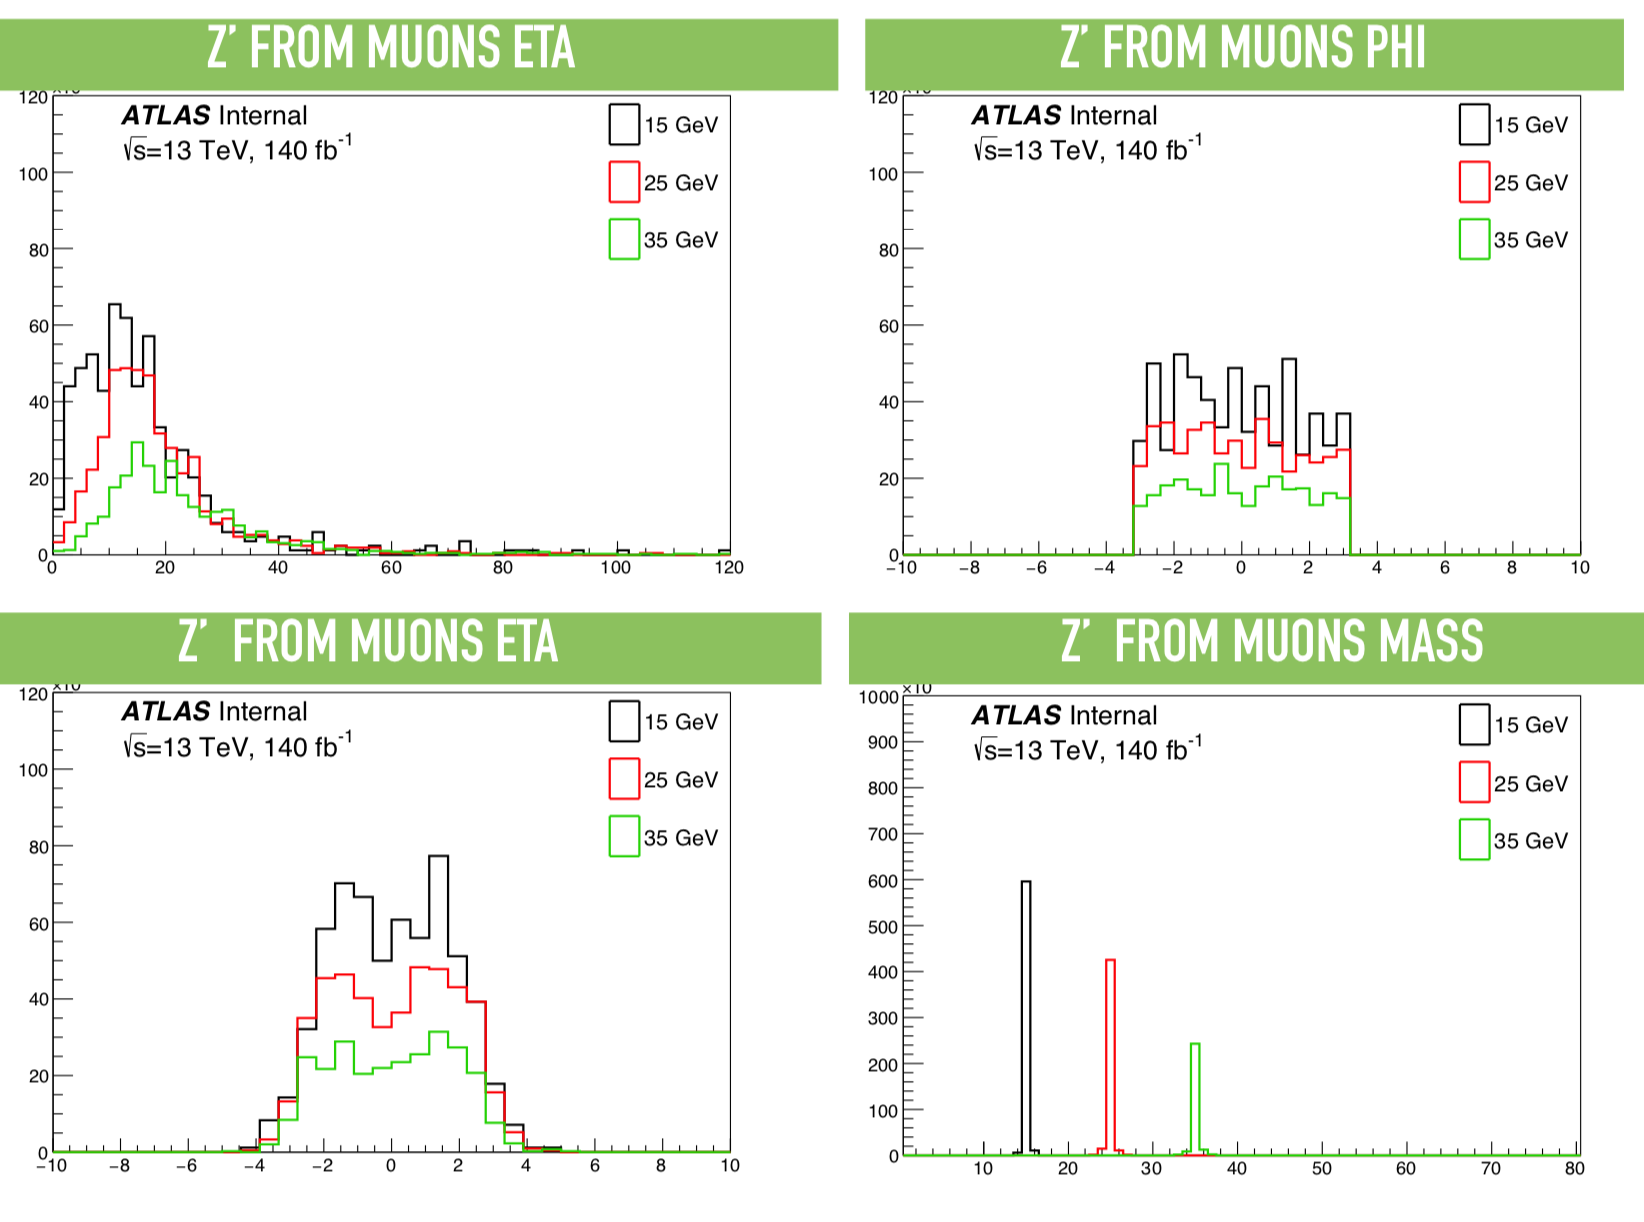
\includegraphics[width=0.5\textwidth]{figures/chapter_dimuon/dimuonISRdist3}
        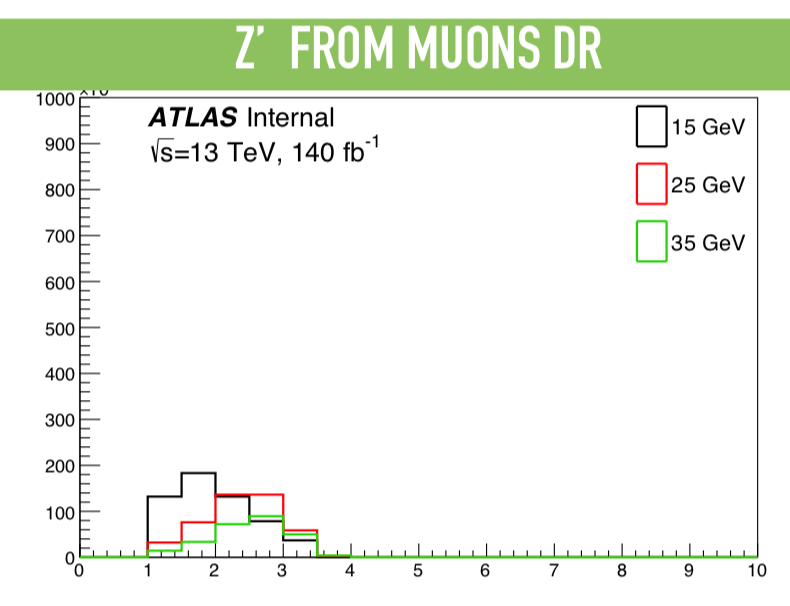
\includegraphics[width=0.2\textwidth]{figures/chapter_dimuon/dimuonISRdist4}
        \caption{
        This figure shows the signal distribution of the boosted dimuon samples generated. A minimal cut of muon pt >14 gev are done on the two leading muons. }
       \label{fig:boosted}
    \end{center}
\end{figure}


\section{Data preparation}

\subsection{Samples Used for the Analysis}
The following are the samples used for the analysis.

\begin{table}[!htb]
    \begin{center}
    \caption{
        The table shows the Monte Carlo dataset used for the analysis. 
    }
\label{tab:MC samples}
\begin{tabular}{|l|l|}
\hline
\textbf{MC Type}   & \textbf{DSID}                                                         \\ \hline
Z+ jets $\mu\mu$   & 364100 - 364113 , 364198-364203                                       \\ \hline
Z+jets $\tau \tau$ & 364128 - 364141 , 364210-364215                                       \\ \hline
$t\bar{t}$         & 410472                                                                \\ \hline
Diboson Sherpa     & 364253 - 364255 , 363355 - 363360 ; 363489 ; 364250 ; 364288 - 364290 \\ \hline
Top decay          & 410644 - 410645 , 410658 - 410659 ; 410648 - 410649                   \\ \hline
W + jets munu      & 364156 - 364169                                                       \\ \hline
$b\bar{b}$         & 363833                                                                \\ \hline
$c\bar{c}$         & 363834                                                                \\ \hline
\end{tabular}
\end{center}
\end{table}


\begin{table}[!htb]
    \begin{center}
    \caption{
        The table shows the Data dataset used for the analysis. 
    }
\label{tab:MC samples}
\begin{tabular}{|l|l|}
\hline
\textbf{Data Taking year}   & \textbf{Data Period} \\ \hline
2015   & D-J                                       \\ \hline
2016   & A-L                                       \\ \hline
2017   & B-F, H                                    \\ \hline
2018   & B-F, I, K, L-O, Q                         \\ \hline
\end{tabular}
\end{center}
\end{table}


\subsection{Trigger Chain}
The analysis takes the "OR" of the three trigger chains :

\begin{itemize}
    \item{HLT\_2mu14}
    \item{HLT\_mu22\_mu8noL1}
    \item{HLT\_mu26\_ivarmedium}
\end{itemize}

\begin{figure}[!htb]
    \begin{center}
        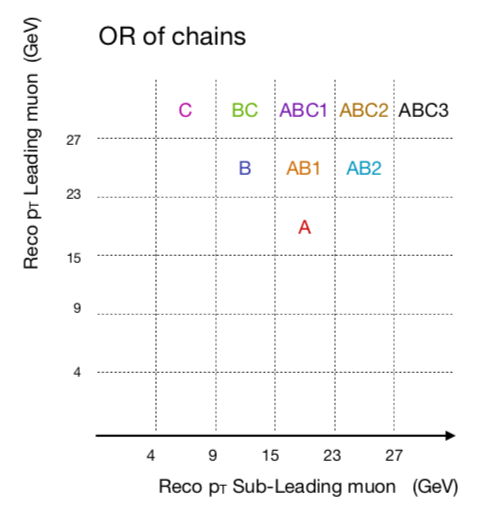
\includegraphics[width=0.75\textwidth]{figures/chapter_dimuon/TriggerChain}        
        \caption{
        This cartoon illstrate the trigger used for the different trigger region. A is HLT\_2mu14, B represents HLT\_mu22\_mu8noL1; C shows HLT\_mu26\_ivarmedium. }
    \end{center}
\end{figure}

%The efficiency are calculated for each region for the subsequent weighting of in the trigger scale factor.
%\begin{equation}
%    SF= \epsilon_{data}/\episilon_{MC}
%\end{equation}

\subsection{Background composition}
The background composition of the Monte Carlo is shown here:

\begin{figure}[!htb]
    \begin{center}
        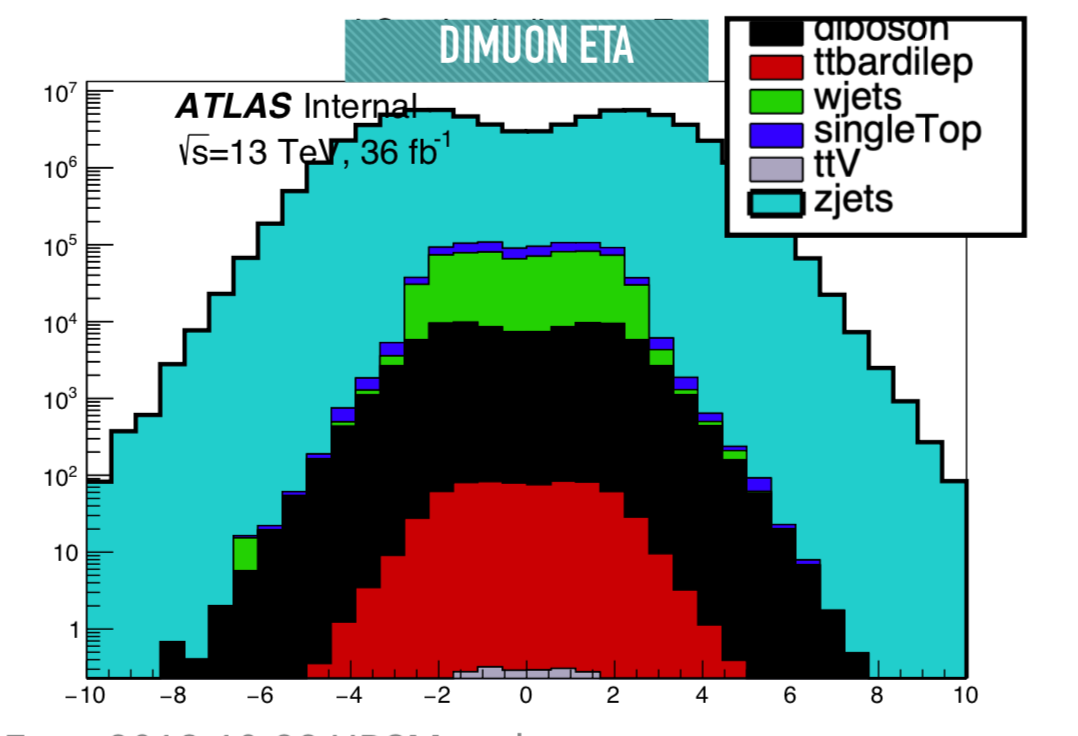
\includegraphics[width=0.75\textwidth]{figures/chapter_dimuon/backgroundcomposition}
        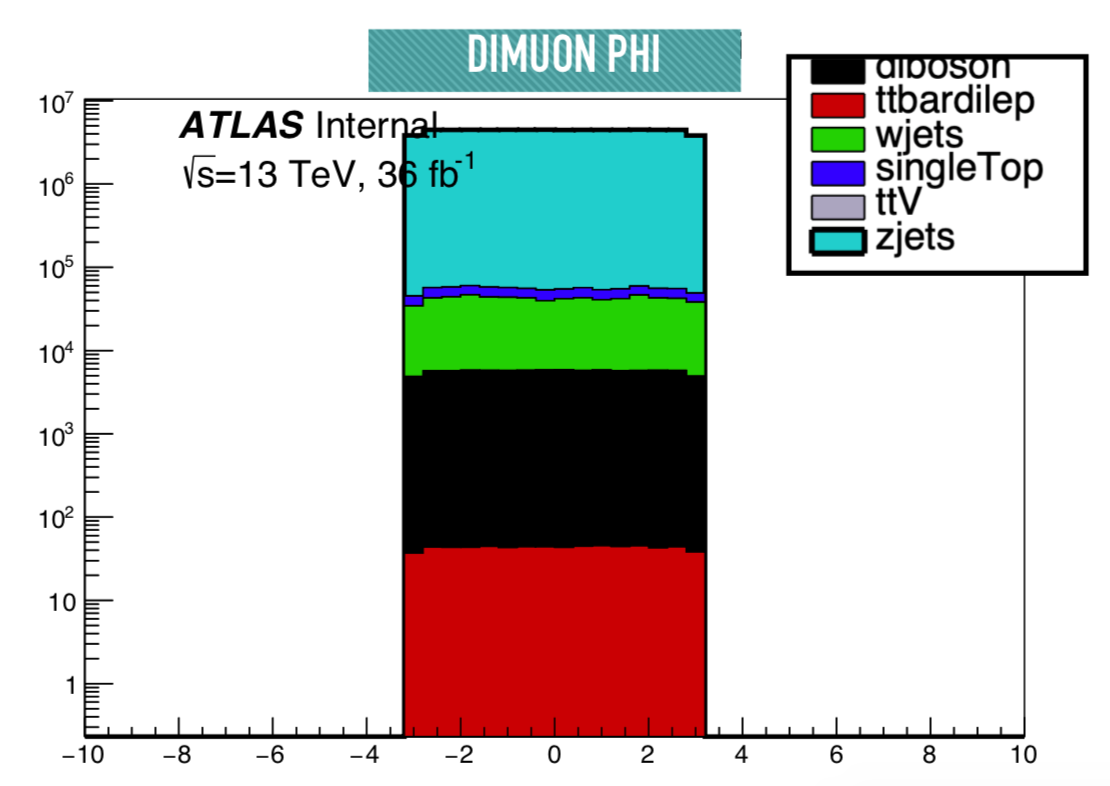
\includegraphics[width=0.75\textwidth]{figures/chapter_dimuon/backgroundcomposition2}
        \caption{
        This cartoon illstrate the background composition of the samples }
    \end{center}
\end{figure}

\subsection{Event Selection}
Following the above trigger cuts, the following event selections are made on the muons:

\subsubsection*{Muon Working Point}
The medium working point is chosen for the muons, details to the working point can be found here: 

The choice is made on the medium working point over low PT, as the trigger threshold effectively cut out most muons below 8GeV. The Low PT working point only has a higher efficiency over the medium working point below  6 GeV. 

\subsubsection*{Isolation Working Point}
FixedCutPflowLoose is chosen to be the isolation working point, details on the working point description can be found here:~\ref{}. 


\subsubsection{Fake Estimation}
Fakes are objects that are not opposite signed dimuon pairs that falls into the selection requirement in data event selection due to misidentifications.
Since the fakes mainly comes from QCD ATLAS processes, the amount from same signed process and opposite signed process are approximately the same. 
Fakes in the background sample can be estimated from the same signed leptons in data. Studies found that the content is less than 1\% of all the background contribution. The estimated same signed leptons contribution is added to the MC background composition.

\begin{figure}[!htb]
    \begin{center}
        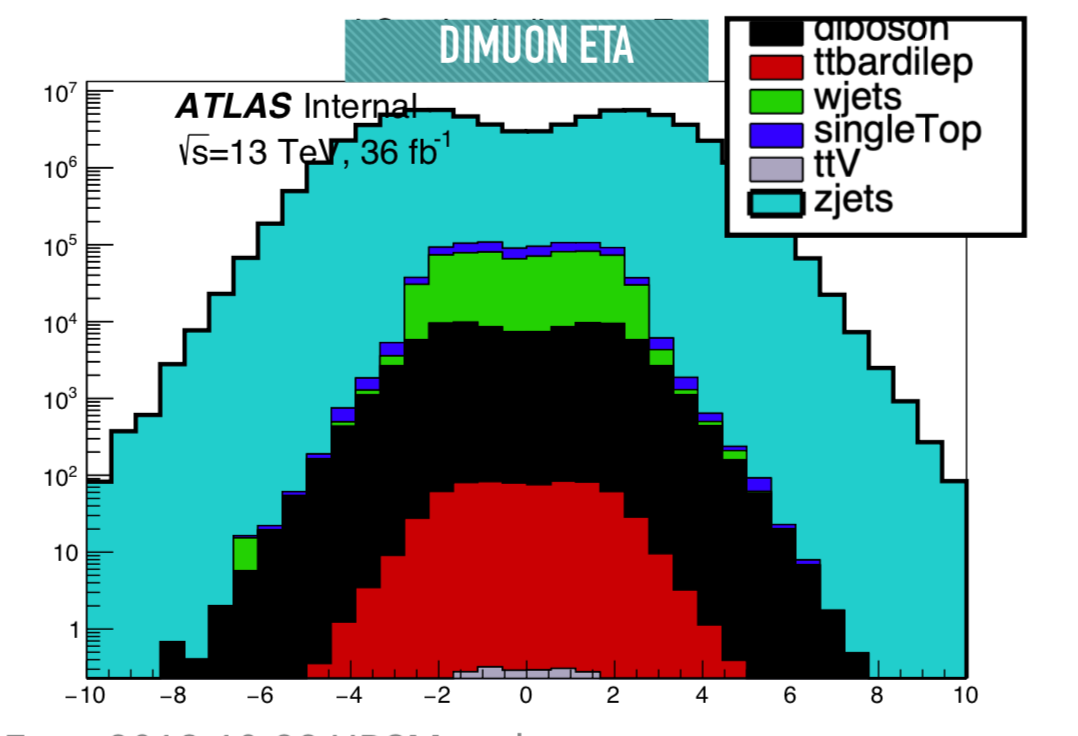
\includegraphics[width=0.75\textwidth]{figures/chapter_dimuon/backgroundcomposition}
        \caption{
        This cartoon illstrating the amount of fakes in the background composition. SS refers to same signed lepton in the data sample set, whereas OS refers to the opposite sign lepton pairs in data. }
    \end{center}
\end{figure}

\subsubsection{Superfast dimuon samples}
Due to the low statistics in the primary background sample in  $Z \> \mu \mu$, fast generation relying on Pythia8 and a smearing function for the detector effect has been used to lower the statistical fluctuation. More details on the fast simulation can be found in the Higgs to $\mu \mu $ int note.

%\subsection{Sensitivity Test}
%Sensitivity test is done on the 

\subsection{Dimuon Mass Spectrum Resolution}
The mass spectrum resolution are done on the Powheg samples of Z > $\mu \mu
$. A Gaussian distribution fit is performed on the resonance mass $m_{\mu\mu_{Truth}} - m_{\mu\mu{Reco}}$ quantity. From the fit, the width of the Gaussian is obtained~\ref{fig:fit}, and is shown to follow the following distribution in figure~\ref{fig:sigma}.
    

\begin{figure}[!htb]
    \begin{center}
        \includegraphics[width=0.75\textwidth]{figures/chapter_dimuon/fitError}        
        \caption{
            A Gaussian distribution fit is made on the the difference between the truth dimuon resonance mass and the reconstructed dimuon resonance mass. }
    \end{center}
\end{figure}
   
\begin{figure}[!htb]
    \begin{center}
        \includegraphics[width=0.75\textwidth]{figures/chapter_dimuon/sigma}        
        \caption{
        From the fitted Gaussian distribution, the width is obtained for different resonance mass. They are plotted here. The width-to-mass resolution $\sigma_{m_{\mu\mu}}/m_{\mu\mu}$ is found to be close to 1.5\%.}
    \end{center}
\end{figure}


\subsection{Binning Strategy}
Using the resolution of the study from the last section and the mass distribution given in the theoretical signal section, the overall binning is chosen to be 0.25 GeV, it will allow for all signal searched for to be at least 2 bin wide. Signal that are at least two bin wide are significantly less prone to accidental "discoveries" due to statistical fluctuation.

\subsubsection{MC/Data Comparison}
A detailed description on the MC/Data comparison test can be found here,\ref{sec:MCData}.  
The agreement is shown to be good between the prepared MC and data. It shows that the MC is ready to be used for the subsequent tests.

\begin{figure}[!htb]
    \begin{center}
        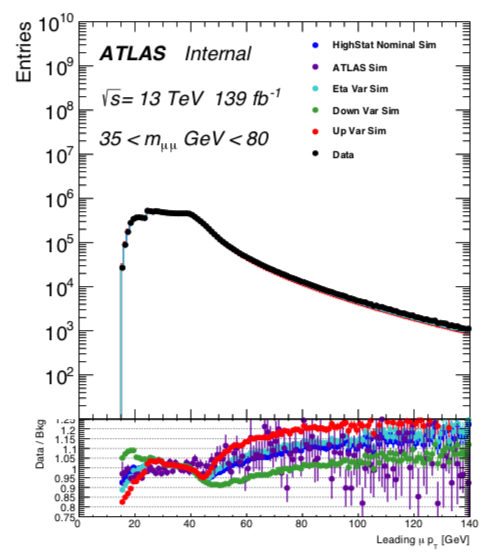
\includegraphics[width=0.75\textwidth]{figures/chapter_dimuon/MCDataCompare}
        %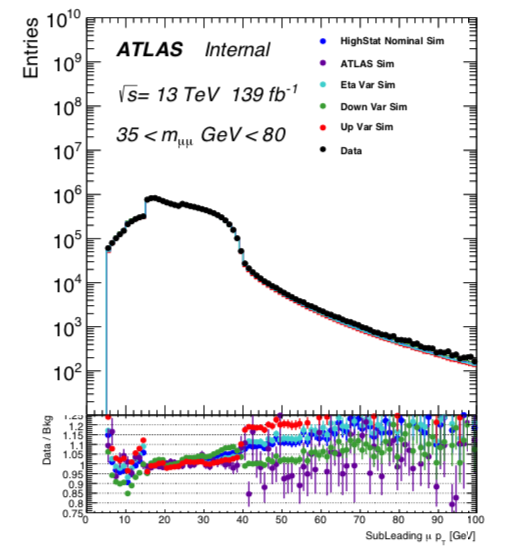
\includegraphics[width=0.75\textwidth]{figures/chapter_dimuon/MCDataCompare2}
        %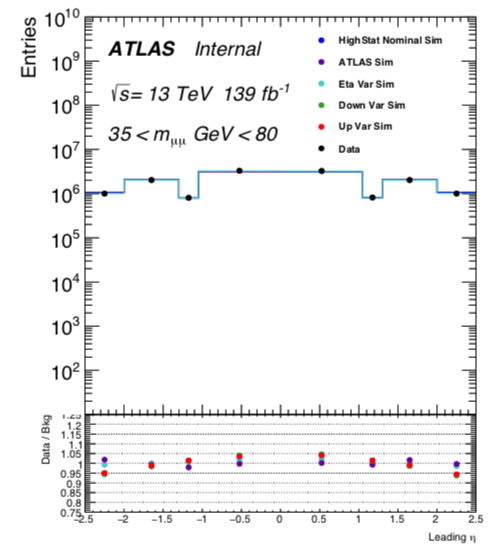
\includegraphics[width=0.75\textwidth]{figures/chapter_dimuon/MCDataCompare3}
        %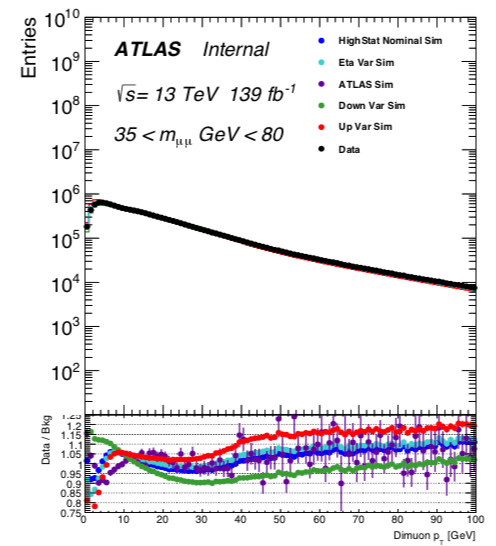
\includegraphics[width=0.75\textwidth]{figures/chapter_dimuon/MCDataCompare4}
        %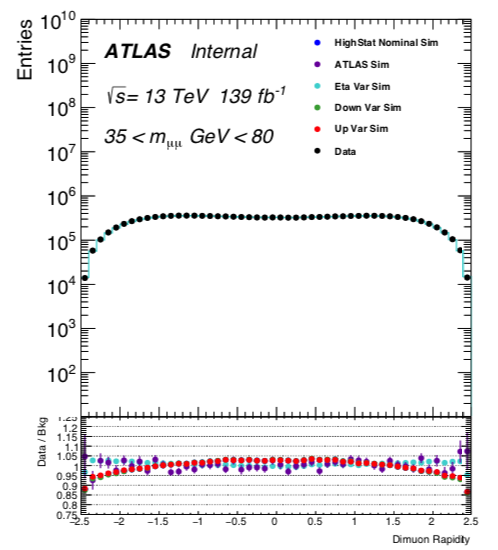
\includegraphics[width=0.75\textwidth]{figures/chapter_dimuon/MCDataCompare5}
        \caption{
        Monte Carlo and data comparison. A reasonable agreement is seen. Showing that the MC is ready to be used for the subsequent studies.
        }
    \end{center}
\end{figure}

\section{Background Fitting}

The Gaussian process background fitting method is being used for this study, a back-up fit function method is also used. Details on how these methods are motivated can be found here~\ref{section:backgroundest}.  

\subsection{Gaussian Process}

The Gaussian process background and signal kernels are given as cited here~\ref{sec:kernel}.

The minimum background lengthscale is studied through the signal injection test described here~\ref{signalInjection}.

Signal of mass widths of 1\%, 3\% and 5\% of different sizes are injected into the mass spectrum. It's found that a minimum lengthscale of 4 GeV is needed for the background kernel for the background model to be sensitive to signal of 3$\sigma$ background error size and above.


\subsubsection{Signal injection test}
\begin{figure}[!htb]
    \begin{center}
        \includegraphics[width=0.75\textwidth]{figures/chapter_dimuon/signalInjection}        
        \caption{
        This figure illustrate a signal injection test performed at the mass point  }
            \label{fig:dimuonstudies}
    \end{center}
\end{figure}

\subsubsection{Background Modelling}
Using the minimal lengthscale chosen for the background and allowing other hyperparameters to float, tests fits are performed on the nominal fit, and also done on the different statistical variation of the background, the 1 $\sigma$ up and 1 $\sigma$ down variation of the fast simulation Pythia, as well as the $\eta$ variation.
The fitting result shows that Gaussian Process works well for all of these statistical variations. 

\begin{figure}[!htb]
    \begin{center}
        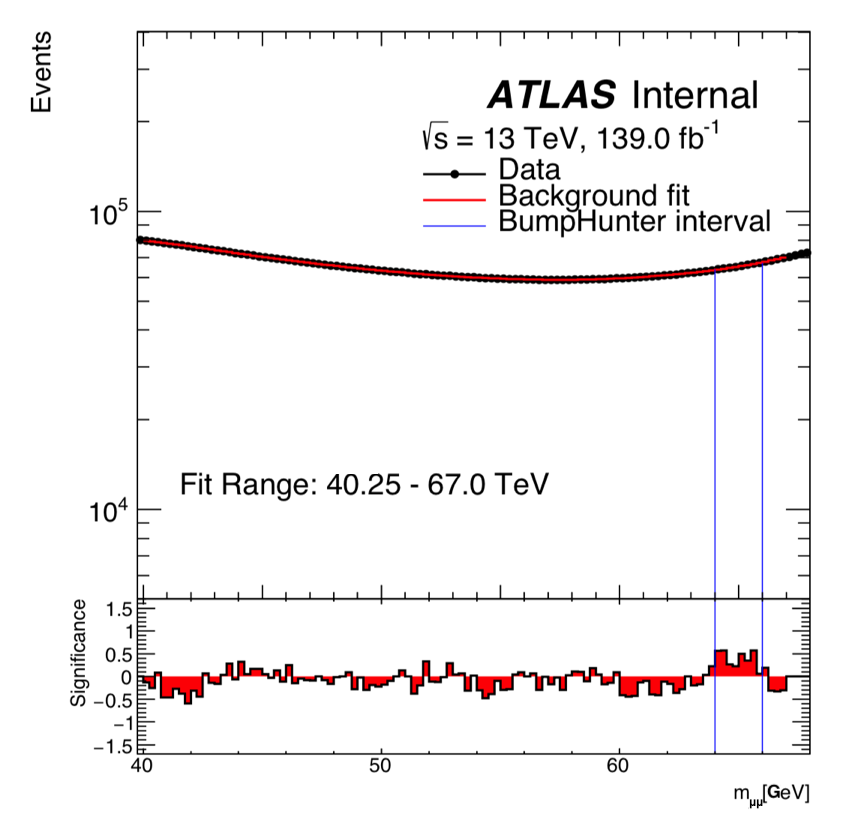
\includegraphics[width=0.75\textwidth]{figures/chapter_dimuon/Nominal}        
        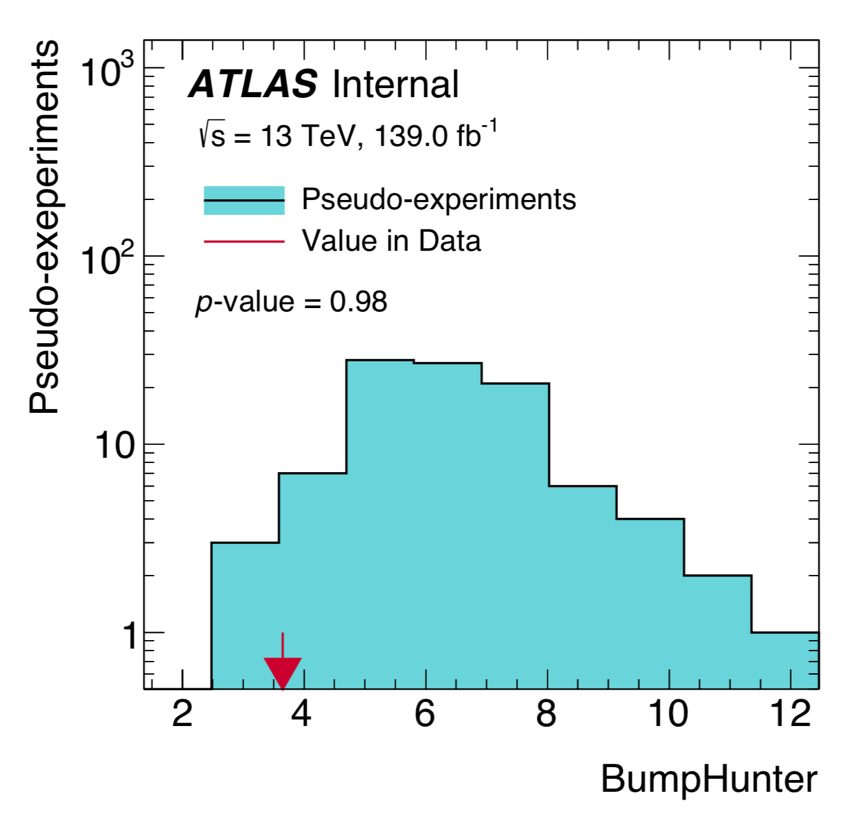
\includegraphics[width=0.75\textwidth]{figures/chapter_dimuon/NominalBH}        
        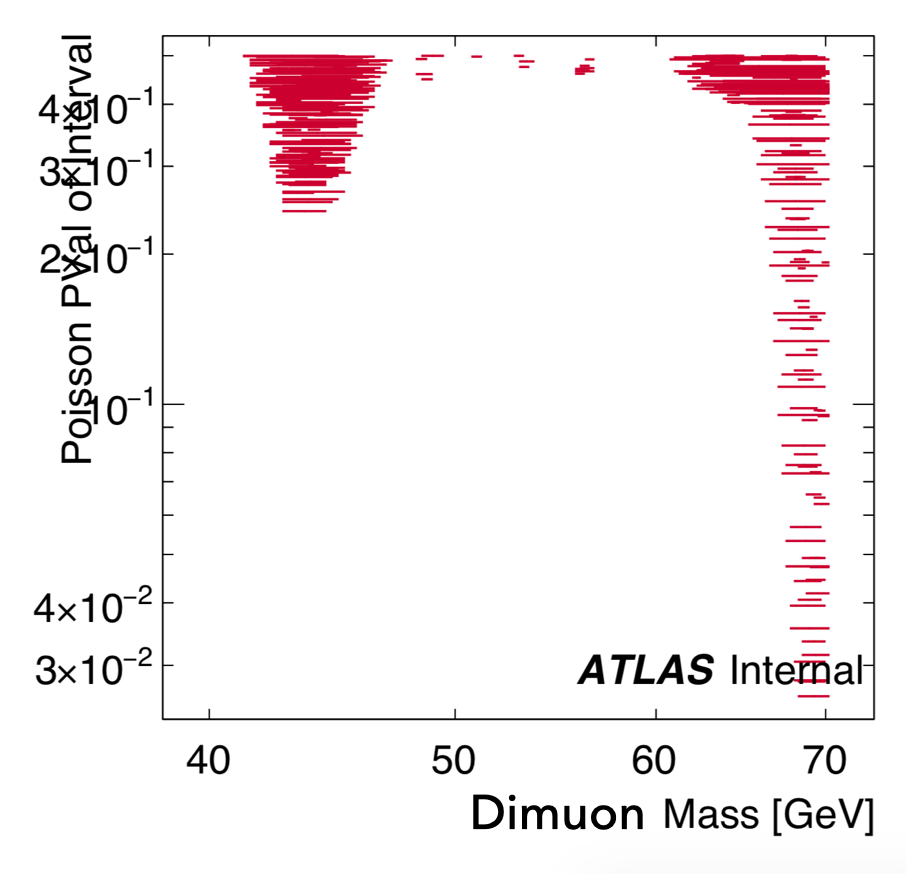
\includegraphics[width=0.75\textwidth]{figures/chapter_dimuon/NominalFit}        
        \caption{
        These figure illustrates the nominal fit, along with the bumphunter test statistics and the observed value distribution. It's shown that the most discrepant window does not fall below the critical p-value of 0.01. Details on the bumphunting procedure can be found here. }
            \label{fig:dimuonstudies}
    \end{center}
\end{figure}


\begin{figure}[!htb]
    \begin{center}
        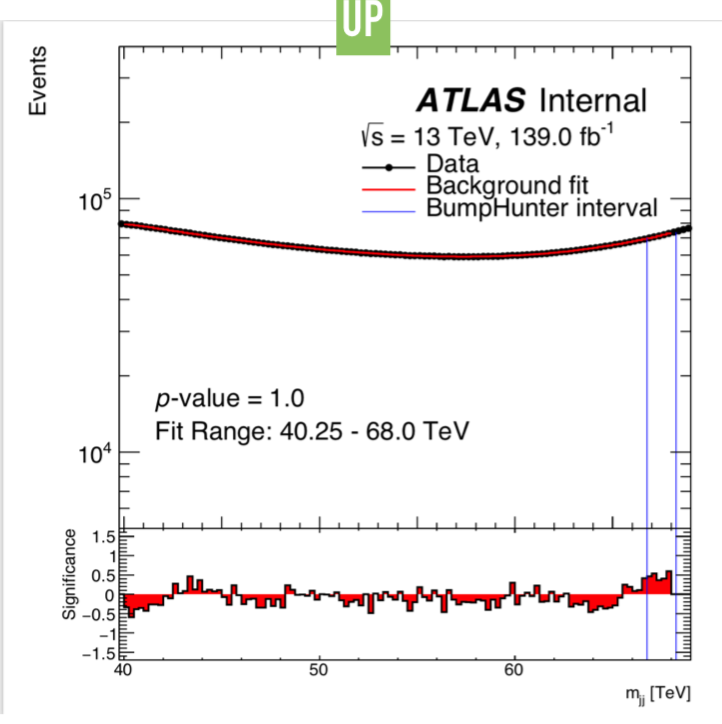
\includegraphics[width=0.75\textwidth]{figures/chapter_dimuon/UpVariation}
        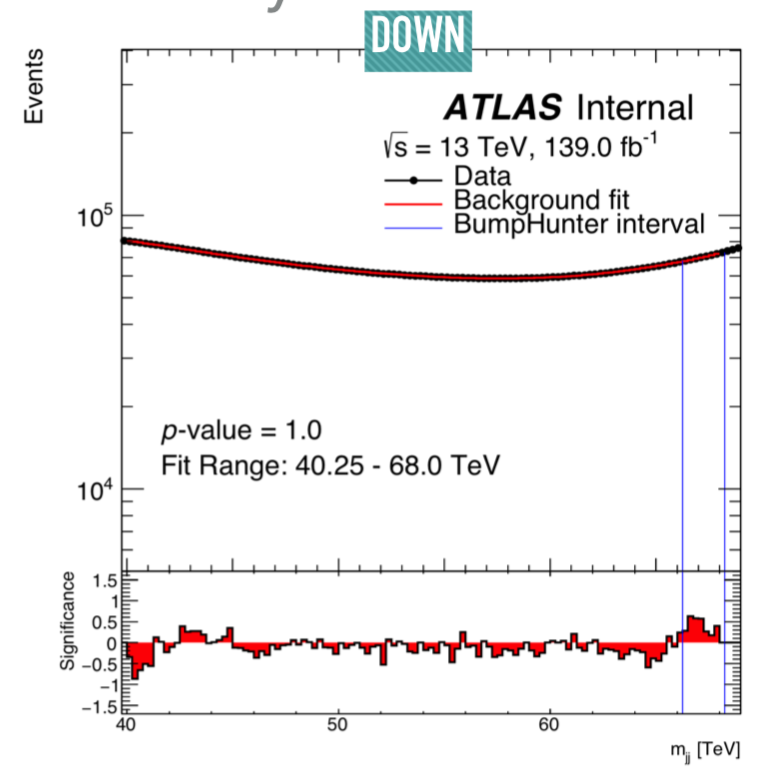
\includegraphics[width=0.75\textwidth]{figures/chapter_dimuon/DownVariation}
        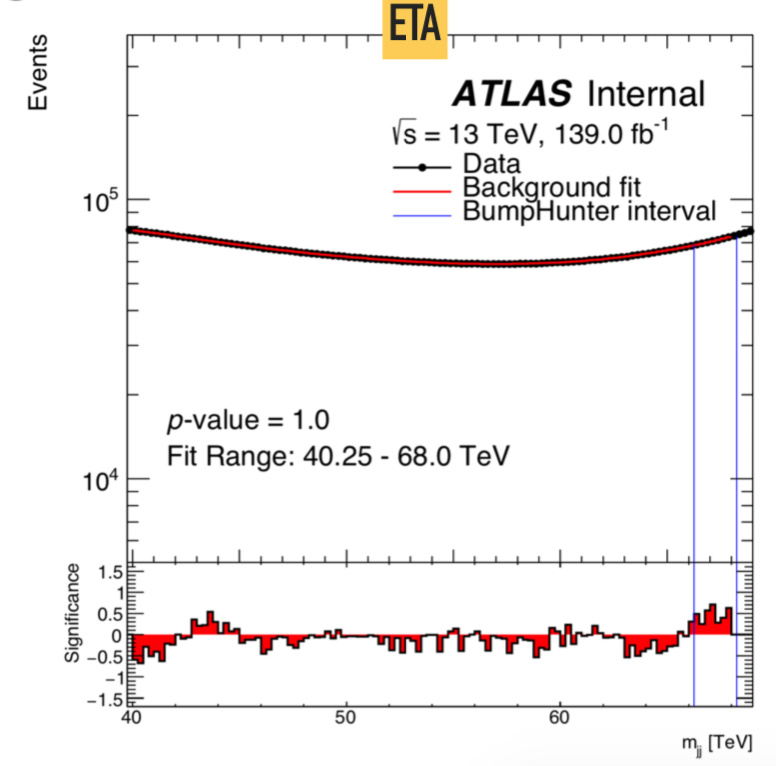
\includegraphics[width=0.75\textwidth]{figures/chapter_dimuon/EtaVariation}
        \caption{
        These figure illustrates the Gaussian Process background fits on the different variation of the MC generated. }
    \end{center}
\end{figure}



\subsection{Spurious signal test}
Details on the spurious signal can be found here~\ref{spurious}.
The spurious signal test results on the Gaussian process is shown here:

\begin{figure}[!htb]
    \begin{center}
        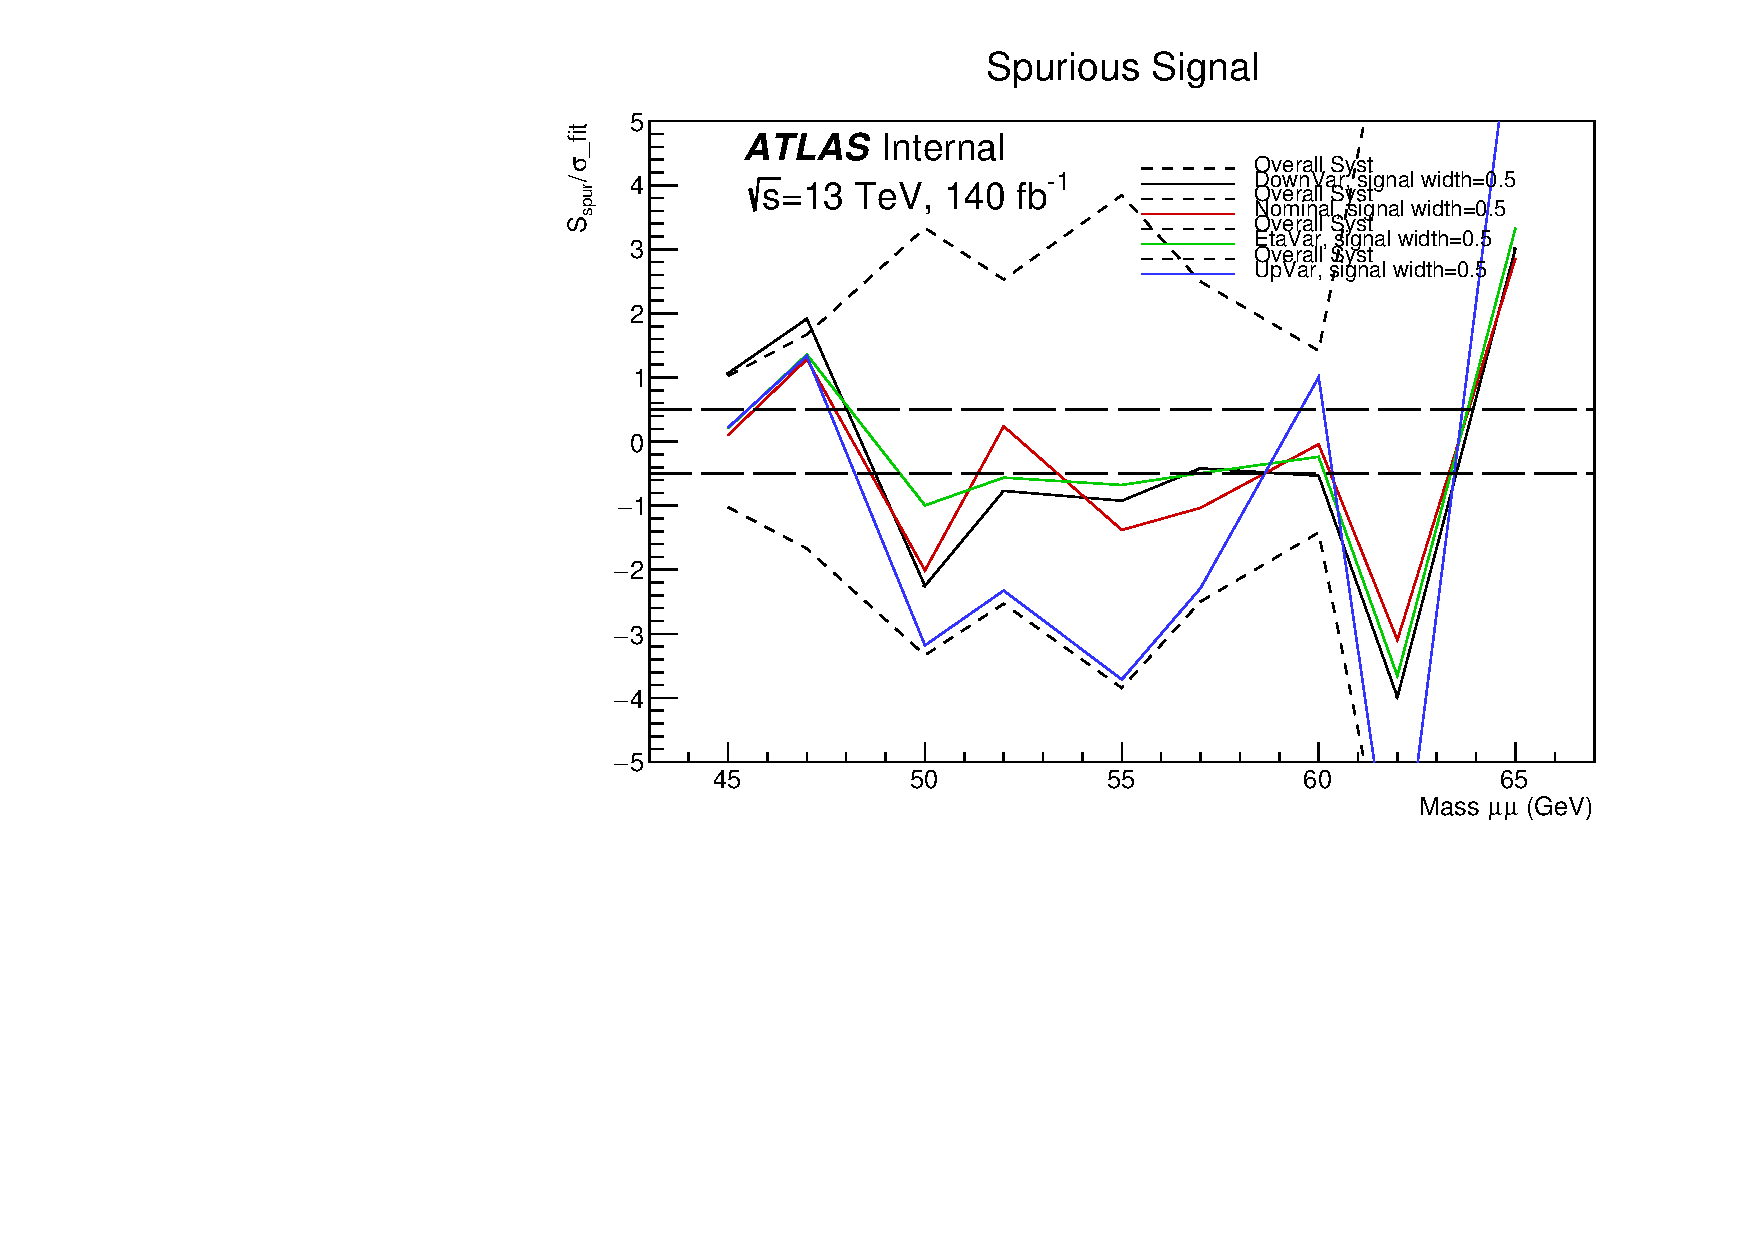
\includegraphics[width=0.75\textwidth]{figures/chapter_dimuon/spurious}        
        \caption{
        This figure illustrate a spurious signal test result on the different background variation fits.}
            \label{fig:dimuonstudies}
    \end{center}
\end{figure}

\section{Statistics Testing}
Details on the statistical test can be found here~\ref{}. During the time where the thesis was written, the data was not unblinded. Monte Carlo studies were done. A sample signal is injected into the spectrum to test the bumphunter, and the limit is generated using background MC assuming no signal was found.

\section{
The Search}
A sample signal the size of 3$\sigma$ background error is injected into the spectrum, the test is done to illustrate that the search is capable of picking out the signal.
    
\begin{figure}[!htb]
    \begin{center}
        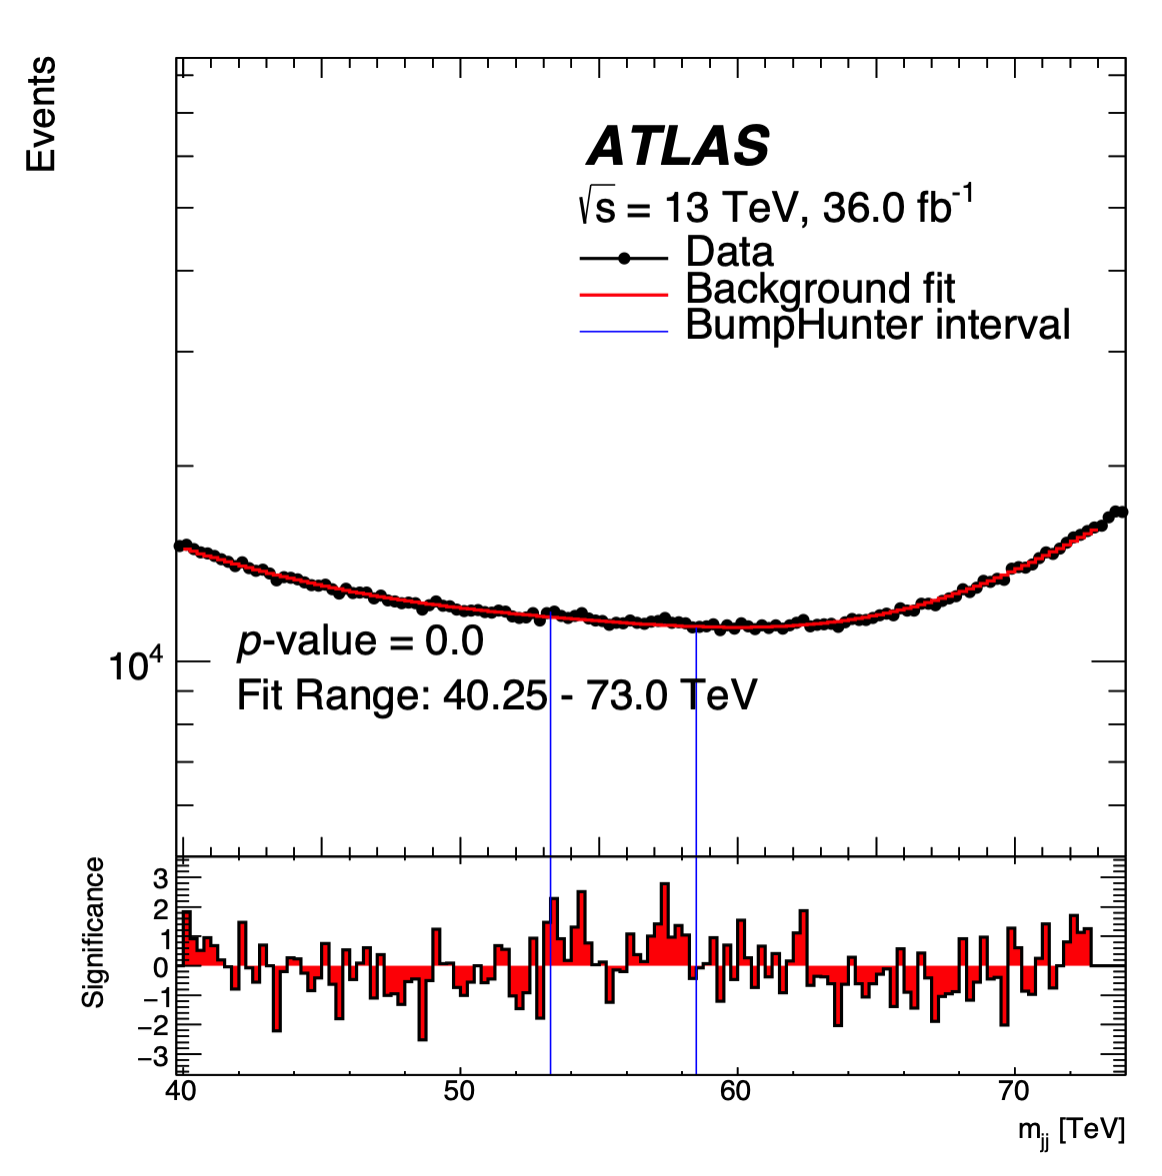
\includegraphics[width=0.75\textwidth]{figures/chapter_dimuon/signalinjected}
        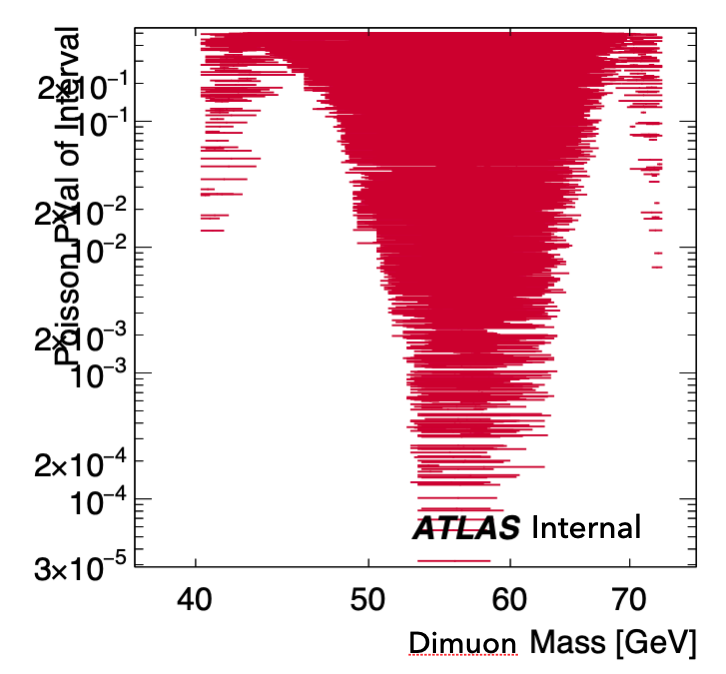
\includegraphics[width=0.75\textwidth]{figures/chapter_dimuon/signalinjected2}
        \caption{
        These figures illustrate a test done on signal injected at 55 GeV, and the window exclusion that picked out the signal injected in there.}
%            \label{fig:dimuonstudies}
    \end{center}
\end{figure}

\section{Limit Setting}
Preliminary limit setting is still currently under test, figure\ref{} shows a preliminary result from the Asimov method. 

\begin{figure}[!htb]
   \begin{center}
       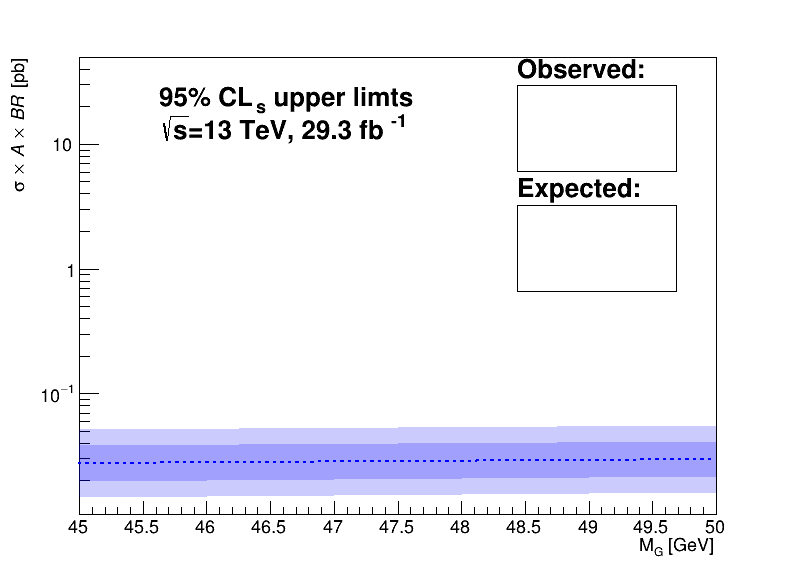
\includegraphics[width=0.75\textwidth]{figures/chapter_dimuon/limits}       
       \caption{
       This figure illustrate a spurious signal test result on the different background variation fits.
       }
    \label{fig:dimuonstudies}
   \end{center}
\end{figure}

In alternative fit function limits calculated by approximation based on the fit function method is shown here, it's expected that the analysis will have comparible sensitivity to LHCb. 

\begin{figure}[!htb]
   \begin{center}
       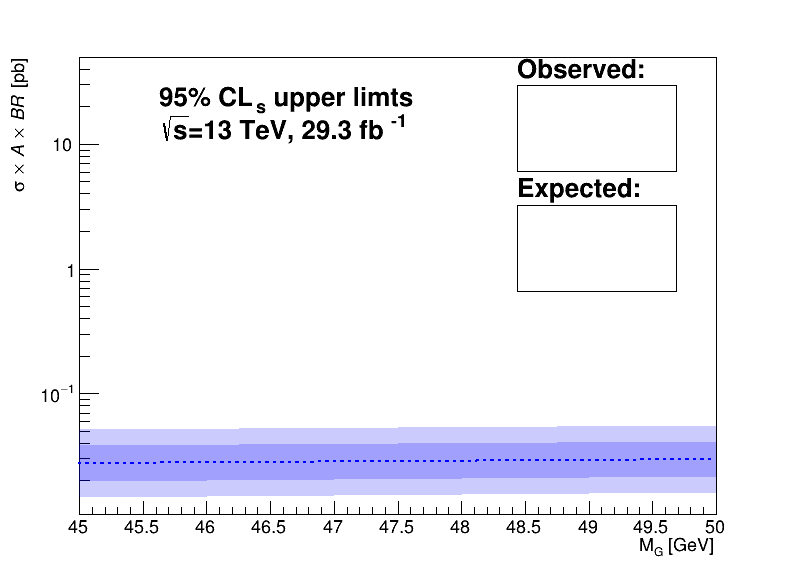
\includegraphics[width=0.75\textwidth]{figures/chapter_dimuon/limits}
       \caption{
       This figure illustrate a spurious signal test result on the different background variation fits.}
            \label{fig:dimuonstudies}
   \end{center}
\end{figure}



\section{Future Work}
The analysis is on its way to completing the final strategies and to be unblinded on data soon.

\section{Alternative fitting}
An alternative fitting method is done through the fit function method.

\section{Systematics}
section{Future Extensions}

